% !TEX root = task-21.tex
% EGE 2027, task 21. Source IDs and URLs are kept in comments.
% Editable task bank. Append new BankTask blocks at the end of the document.
\documentclass[12pt,a4paper]{article}
\usepackage{physics-textbook}
\usepackage{graphicx,needspace}
\usetikzlibrary{decorations.pathmorphing}
\newif\ifShowSolutions
\ifdefined\TutorEdition
  \ShowSolutionstrue
\else
  \ShowSolutionsfalse % Change to \ShowSolutionstrue to display solutions.
\fi
\newcounter{banktask}
\newsavebox{\BankTaskBox}
\newcommand{\BankTaskContent}[3]{%
  \noindent\textbf{\thebanktask.}\quad #2\par
  \ifShowSolutions
    \Needspace{50mm}% Keep the solution heading with its opening text or diagram.
    #3\par
    \ifdefined\TutorEdition
      \ifcsname TutorSource#1\endcsname
        \nopagebreak\smallskip{\small\csname TutorSource#1\endcsname\par}%
      \fi
    \fi
  \fi
}
\newcommand{\BankTask}[3]{%
  \refstepcounter{banktask}\par\medskip
  \sbox{\BankTaskBox}{\begin{minipage}{\linewidth}%
    \BankTaskContent{#1}{#2}{#3}\end{minipage}}%
  \ifdim\dimexpr\ht\BankTaskBox+\dp\BankTaskBox\relax>\dimexpr\textheight-20mm\relax
    \Needspace{35mm}\BankTaskContent{#1}{#2}{#3}%
  \else
    \Needspace{\dimexpr\ht\BankTaskBox+\dp\BankTaskBox\relax}%
    \noindent\usebox{\BankTaskBox}\par
  \fi
  \medskip
}
\begin{document}


% Source 51472: https://phys-ege.sdamgia.ru/problem?id=51472
\BankTask{51472}{
\begin{center}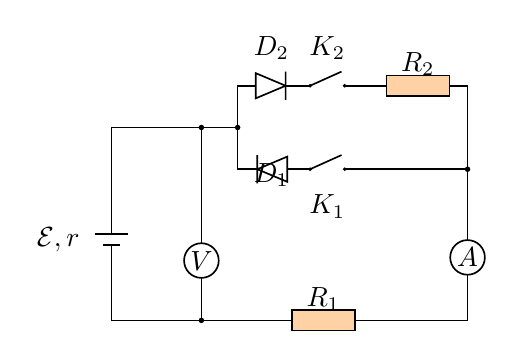
\begin{tikzpicture}[>=stealth,line width=.6pt]

\draw (0,1.1)--(0,2.45)--(1.6,2.45)--(1.6,2.98)--(1.83,2.98)
      (0,.96)--(0,0)--(2.29,0) (3.09,0)--(4.52,0)--(4.52,.58)
      (4.52,1.02)--(4.52,2.98)--(4.29,2.98)
      (1.6,2.45)--(1.6,1.92)--(1.85,1.92) (2.23,1.92)--(2.52,1.92) (2.96,1.92)--(4.52,1.92)
      (2.21,2.98)--(2.52,2.98) (2.96,2.98)--(3.49,2.98)
      (1.14,2.45)--(1.14,.98) (1.14,.54)--(1.14,0);
\fill(1.14,2.45)circle(.035) (1.6,2.45)circle(.035) (1.14,0)circle(.035) (4.52,1.92)circle(.035);
\begin{scope}[shift={(0,1.03)},rotate=-90]\draw(-.07,-.21)--(-.07,.21) (.07,-.11)--(.07,.11);\end{scope}\node[above right] at (0.12,1.03) {$$};\node[left] at (-.28,1.02) {$\mathcal E,r$};\draw (1.14,0.76)circle(.22) node {$V$};\draw (4.52,0.8)circle(.22) node {$A$};\begin{scope}[shift={(2.69,0)},rotate=0]\draw[fill=orange!35] (-.4,-.13) rectangle (.4,.13);\end{scope}\node[above] at (2.69,0) {$R_1$};\begin{scope}[shift={(3.89,2.98)},rotate=0]\draw[fill=orange!35] (-.4,-.13) rectangle (.4,.13);\end{scope}\node[above] at (3.89,2.98) {$R_2$};\begin{scope}[shift={(2.03,2.98)},rotate=0]\draw(-.2,-.16)--(-.2,.16)--(.18,0)--cycle (.18,-.18)--(.18,.18);\end{scope}\node[above] at (2.03,3.18) {$D_2$};\begin{scope}[shift={(2.03,1.92)},rotate=180]\draw(-.2,-.16)--(-.2,.16)--(.18,0)--cycle (.18,-.18)--(.18,.18);\end{scope}\node[below] at (2.03,2.12) {$D_1$};\begin{scope}[shift={(2.74,2.98)},rotate=0]\draw(-.22,0)--(.18,.18);\fill(-.22,0)circle(.025) (.22,0)circle(.025);\node[above]at(0,.2){$K_2$};\end{scope}\begin{scope}[shift={(2.74,1.92)},rotate=0]\draw(-.22,0)--(.18,.18);\fill(-.22,0)circle(.025) (.22,0)circle(.025);\node[above]at(0,.2){$$};\end{scope}\node[below] at (2.74,1.72) {$K_1$};
\end{tikzpicture}\end{center}
На рисунке изображена электрическая цепь, состоящая из гальванического элемента, двух идеальных диодов (сопротивление диода при прямом включении равно нулю, при обратном включении ток через диод равен нулю), двух ключей, двух резисторов, идеальных амперметра и вольтметра. 
В начальный момент времени ключ К$_{1}$ замкнут, а ключ К$_{2}$ разомкнут. Опираясь на законы электродинамики, объясните, как изменятся показания приборов, если ключ К$_{1}$ разомкнуть, а ключ К$_{2}$ замкнуть.
}{
\smallskip\noindent\textbf{Решение}\par
$1$.  В начальный момент времени, когда ключ К$_{1}$ замкнут, а ключ К$_{2}$ разомкнут, диод D$_{1}$ закрыт, ток в цепи и токи через диоды отсутствуют. Ток через амперметр не течёт, то есть $I_1 = 0,$ и показания прибора равны нулю. Вольтметр показывает $U_1 = \mathcal{E}.$
$2$.  Если ключ К$_{1}$ разомкнуть, а ключ К$_{2}$ замкнуть, то ток пойдёт через диод D$_{2}$  — он открыт  — и резистор R$_{2}$. В соответствии с законом Ома для полной цепи сила тока $I_2 = \frac{\mathcal{E}}{R_{\,\text{общ}} + r} ,$ где общее сопротивление при последовательном соединении проводников равно $R_{\,\text{общ}}=R_1 + R_2.$ Амперметр во втором случае покажет силу тока $I_2 = \frac{\mathcal{E}}{R_1 + R_2 + r} .$ Следовательно, показания амперметра увеличатся.
$3$.  При этом напряжение, которое показывает вольтметр, в соответствии с законом Ома для участка цепи станет $U_2 = I_2R_{\,\text{общ}}$ и законом Ома для полной цепи

\[U_2 = \mathcal{E} - I_2 r.\]

 Показания вольтметра уменьшатся.

Ответ: показания вольтметра уменьшатся, а показания амперметра увеличатся.
}

% Source 4508: https://phys-ege.sdamgia.ru/problem?id=4508
\BankTask{4508}{
К колебательному контуру подсоединили источник тока, на клеммах которого напряжение гармонически меняется с частотой $\nu.$ Электроемкость С конденсатора колебательного контура можно плавно менять от минимального значения $C_{\min}$ до максимального $C_{\max},$ а индуктивность его катушки постоянна. Ученик постепенно увеличивал емкость конденсатора от минимального значения до максимального и обнаружил, что амплитуда силы тока в контуре все время возрастала. Опираясь на свои знания по электродинамике, объясните наблюдения ученика.
}{
\smallskip\noindent\textbf{Решение}\par
В колебательном контуре источником тока возбуждаются вынужденные колебания. Частота этих колебаний равна частоте источника $\nu.$ Амплитуда же зависит от соотношения между внешней частотой и частотой собственных электромагнитных колебаний $\nu_0 = \frac{1}{2 \pi \sqrt{LC}} .$ По мере увеличения емкости конденсатора уменьшается частота собственных колебаний в колебательном контуре. Амплитуда колебаний достигает максимума при резонансе, когда $\nu=\nu_0.$ После этого амплитуда начинает убывать. В данном случае, ученик меняет не внешнюю частоту, а частоту собственных электромагнитных колебаний. При плавном увеличении емкости контура от минимального значения $C_{\min}$ до максимального $C_{\max},$ частота уменьшается от $\nu_0,\max = \frac{1}{2 \pi \sqrt{LC_{\min}}}$ до $\nu_0,\min = \frac{1}{2 \pi \sqrt{LC_{\max}}} .$ Из того факта, что амплитуда все время увеличивалась, можем сделать вывод, что частота $\nu_0$ все время приближалась к частоте источника тока, при этом $\nu < \nu_0,\min.$
}

% Source 38568: https://phys-ege.sdamgia.ru/problem?id=38568
\BankTask{38568}{
\begin{center}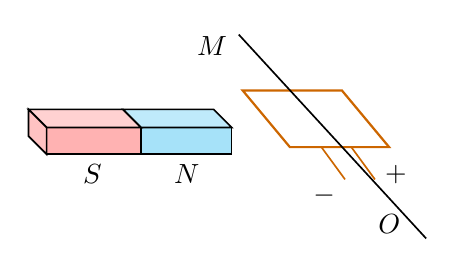
\begin{tikzpicture}[>=stealth,line width=.6pt]

\filldraw[fill=red!30](-3.2,.16)rectangle(-2,.5);
\filldraw[fill=cyan!35](-2,.16)rectangle(-.85,.5);
\filldraw[fill=red!18](-3.2,.5)--(-3.43,.73)--(-2.23,.73)--(-2,.5)--cycle;
\filldraw[fill=cyan!25](-2,.5)--(-2.23,.73)--(-1.08,.73)--(-.85,.5)--cycle;
\filldraw[fill=red!24](-3.2,.16)--(-3.43,.39)--(-3.43,.73)--(-3.2,.5)--cycle;
\node[below] at (-2.62,.16) {$S$};\node[below] at (-1.42,.16) {$N$};
\draw[orange!80!black,thick](-.71,.97)--(.55,.97)--(1.15,.25)--(-.11,.25)--cycle;
\draw[orange!80!black] (.29,.25)--(.59,-.16) (.67,.25)--(.97,-.16);
\draw(-.76,1.68)--(1.62,-.91);
\node[left]at(-.78,1.53){$M$};\node[left]at(1.42,-.73){$O$};
\node[below left]at(.59,-.12){$-$};\node[right]at(.97,-.1){$+$};

\end{tikzpicture}\end{center}
Рамку с постоянным током удерживают неподвижно в поле полосового магнита (см. рис.). Полярность подключения источника тока к выводам рамки показана на рисунке. Как будет двигаться рамка на неподвижной оси MО, если рамку не удерживать? Ответ поясните, указав, какие физические закономерности вы использовали для объяснения. Считать, что рамка испытывает небольшое сопротивление движению со стороны воздуха.
}{
\smallskip\noindent\textbf{Решение}\par
Линии магнитного поля, созданного постоянным магнитом, направлены вправо. По рамке течет ток от плюса к минусу. Выясним направление силы Ампера, с которой магнитное поле действует на каждую сторону данной рамки. В дальней от магнита стороне рамки ток течет в плоскость рисунка. По правилу левой руки сила Ампера направлена вертикально вниз. В ближней от магнита стороне рамки ток течет из плоскости рисунка. По правилу левой руки сила Ампера направлена вертикально вверх. На горизонтальные стороны рамки сила Ампера не действует, так как угол между вектором магнитной индукции и направлением тока равен $0^\circ$ или $180^\circ$, для которых  $\sin \alpha = 0$  и сила Ампера $F_A=BIl \sin \alpha =0.$
В результате действия противоположно направленных сил на стороны рамки она будет поворачиваться по часовой стрелке, двигаясь замедленно из-за сопротивления воздуха. Кроме того, при повороте рамки на угол чуть больший $90^\circ$ силы Ампера будут рамку тормозить. В результате рамка расположится вертикально, ее плоскость будет перпендикулярна магнитным линиям.
}

% Source 25398: https://phys-ege.sdamgia.ru/problem?id=25398
\BankTask{25398}{
Маленький незаряженный шарик, подвешенный на непроводящей нити, помещен над горизонтальной диэлектрической пластиной, равномерно заряженной положительным зарядом. Размеры пластины во много раз превышают длину нити. Опираясь на законы механики и электродинамики, объясните, как изменится частота малых свободных колебаний шарика, если ему сообщить отрицательный заряд.
}{
\smallskip\noindent\textbf{Решение}\par
При отсутствии заряда шарика частота его колебаний определяется формулой

\[v = \frac{1}{T} = \frac{1}{2 \pi} \sqrt{\frac{g}{l}} .\]


\begin{center}\begin{tikzpicture}[>=stealth,line width=.6pt]

\draw(-.36,2.97)--(.36,2.97);
\foreach \x in {-.33,-.24,...,.33}{\draw(\x,2.97)--++(.14,.14);}
\draw(0,2.97)--(.14,0) node[midway,left] {$l$};
\draw(0,2.97)--(.91,.11);
\filldraw[fill=orange!45,draw=orange!85!black] (.14,0)circle(.12) (.91,.11)circle(.12);
\draw[->](.14,0)--(2.01,.26) node[midway,below left] {$x$};
\draw[->,thick](.91,.11)--(.67,.87)node[above left]{$\vec T$};
\draw[->,thick](.88,.11)--(.88,-.65)node[below left]{$\vec F_{\text{э}}$};
\draw[->,thick](.94,.11)--(.94,-.91)node[below right]{$m\vec g$};
\fill(.91,.11)circle(.035);

\end{tikzpicture}\end{center}

Если шарик зарядить, то на него со стороны заряженной пластины будет действовать электрическая сила, направленная вертикально вниз, так как пластина имеет положительный заряд, а шарик отрицательный.
Маятник совершает малые колебания, которые являются гармоническими. Потому равнодействующая сила пропорциональна смещению $\,\text{х},$ то есть $F_x= - kx,$ и имеет период колебаний, который находится по формуле $T=2 \pi \sqrt{\frac{m}{k}} ,$ где k  — коэффициент пропорциональности.
Равнодействующая сила равна $\vec F=\vec F_{\,\text{э}} + m\vec{g} + \vec{T},$ ее проекция на ось Ох $F_x= - ( F_{\,\text{э}} + mg ) \cdot \sin \alpha .$
Для малых колебаний можно считать, что $\sin \alpha \approx \frac{x}{l} .$ Тогда 

\[F_x= - ( F_{\,\text{э}} + mg ) \cdot \frac{x}{l} = - \frac{mg + F_{\,\text{э}}}{l} x.\]

Следовательно, коэффициент пропорциональности $k= \frac{F_{\,\text{э}} + mg}{l} .$ В этом случае период колебаний равен

$T=2 \pi \sqrt{\frac{ml}{mg + F_{\,\text{э}}}} ,$ а частота 

$v = \frac{1}{2 \pi} \sqrt{\frac{mg + F_{\,\text{э}}}{ml}} = \frac{1}{2 \pi} \sqrt{\frac{g}{l} + \frac{F_{\,\text{э}}}{ml}} .$

Сравнивая частоту колебаний в обоих случаях, делаем вывод, что она увеличилась.

Ответ: увеличилась.
}

% Source 29735: https://phys-ege.sdamgia.ru/problem?id=29735
\BankTask{29735}{
\begin{center}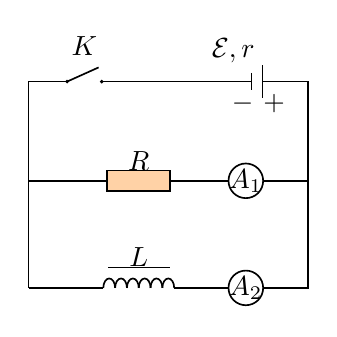
\begin{tikzpicture}[>=stealth,line width=.6pt]

\draw(0,0)--(0,2.62)--(.49,2.62) (.93,2.62)--(2.83,2.62) (2.97,2.62)--(3.55,2.62)--(3.55,0)--(2.98,0)
 (2.54,0)--(1.85,0) (.95,0)--(0,0) (0,1.36)--(1,1.36) (1.8,1.36)--(2.54,1.36) (2.98,1.36)--(3.55,1.36);
\draw(1.01,.26)--(1.8,.26);
\begin{scope}[shift={(0.71,2.62)},rotate=0]\draw(-.22,0)--(.18,.18);\fill(-.22,0)circle(.025) (.22,0)circle(.025);\node[above]at(0,.2){$K$};\end{scope}\begin{scope}[shift={(2.9,2.62)},rotate=180]\draw(-.07,-.21)--(-.07,.21) (.07,-.11)--(.07,.11);\end{scope}\node[above right] at (3.02,2.62) {$$};\node[above] at (2.6,2.73) {$\mathcal E,r$};\node[below] at (2.72,2.59) {$-$};\node[below] at (3.12,2.59) {$+$};\begin{scope}[shift={(1.4,1.36)},rotate=0]\draw[fill=orange!35] (-.4,-.13) rectangle (.4,.13);\end{scope}\node[above] at (1.4,1.36) {$R$};\begin{scope}[shift={(1.4,0)}]\foreach \x in {-.45,-.3,-.15,0,.15,.3}{\draw(\x,0)arc(180:0:.075 and .12);}\node[above] at (0,.15) {$L$};\end{scope}\draw (2.76,1.36)circle(.22) node {$A_1$};\draw (2.76,0)circle(.22) node {$A_2$};
\end{tikzpicture}\end{center}
 Резистор R и катушка индуктивности L с железным сердечником подключены к источнику тока, как показано на схеме. Первоначально ключ K замкнут, показания амперметров A$_{1}$ и A$_{2}$ равны, соответственно, $I_1=1 A$ и $I_2=0{,}1A.$ Что произойдет с величиной и направлением тока через резистор после размыкания ключа K? Ответ поясните, указав, какие явления и законы вы использовали для объяснения.
}{
\smallskip\noindent\textbf{Решение}\par
$1$.  При замкнутом ключе катушка и резистор соединены параллельно, токи в них будут иметь одинаковые направления. Исходя из схемы, токи текут от плюса к минусу, то есть справа налево. 
$2$.  После размыкания ключа в катушке будет наблюдаться явление самоиндукции, в результате чего в ней возникнет ЭДС самоиндукции $\mathcal E_{si}= - L \frac{\Delta I_2}{\Delta t} ,$ препятствующее уменьшению тока через катушку. Тогда ток через катушку будет иметь прежнее направление. 
$3$.  Так как источник тока отключен, а в цепи возникла ЭДС самоиндукции, то резистор будет подключен последовательно с катушкой. В результате ток через резистор изменит направление на противоположное, то есть будет течь слева направо. 
$4$.  Сразу после размыкания ключа через резистор будет течь такой же ток, как и через катушку. Следовательно, он станет равным I$_{2}$, то есть уменьшится от $1\,\text{А}$ до $0{,}1$ A.

Ответ: ток через резистор сразу после размыкания ключа будет течь вправо с силой тока $0{,}1\,\text{А}$.
}

% Source 9040: https://phys-ege.sdamgia.ru/problem?id=9040
\BankTask{9040}{
На рисунке изображены две электрические цепи. Первая содержит последовательно соединенные источник тока ($1$), реостат, катушку индуктивности и амперметр, а вторая  — проволочный моток, к концам которого присоединен гальванометр, изображенный на рисунке справа. Катушка и моток надеты на железный сердечник ($2$).

\begin{center}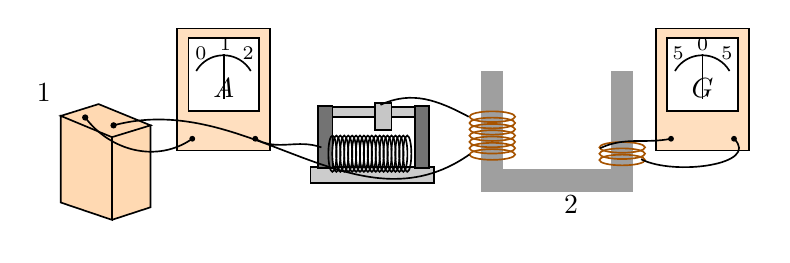
\begin{tikzpicture}[>=stealth,line width=.6pt]

\draw[fill=orange!30] (0,0)--(0,1.1)--(.65,.83)--(.65,-.22)--cycle (.65,.83)--(1.14,.98)--(1.14,-.06)--(.65,-.22) (0,1.1)--(.48,1.25)--(1.14,.98)--(.65,.83)--cycle;
\node[above left] at (0,1.16) {$1$};\fill(.31,1.08)circle(.04) (.67,.98)circle(.04);
\draw[fill=orange!25] (1.48,.66) rectangle (2.66,2.21) (7.56,.66) rectangle (8.74,2.21);
\foreach \x/\s in {2.07/A,8.15/G}{\draw[fill=white](\x-.45,1.16)rectangle(\x+.45,2.09);\draw(\x-.35,1.67) arc(150:30:.4);\draw(\x,1.32)--(\x,1.88);\node at(\x,1.45){$\s$};\fill(\x-.4,.81)circle(.037) (\x+.4,.81)circle(.037);}
\node at(1.78,1.9){\scriptsize $0$};\node at(2.09,2.01){\scriptsize $1$};\node at(2.38,1.9){\scriptsize $2$};
\node at(8.15,2.01){\scriptsize $0$};\node at(7.84,1.9){\scriptsize $5$};\node at(8.46,1.9){\scriptsize $5$};
\draw[fill=gray!40](3.17,.25)rectangle(4.74,.45) (3.29,1.09)rectangle(4.62,1.21);
\draw[fill=black!55](3.27,.44) rectangle(3.45,1.23) (4.5,.44)rectangle(4.68,1.23);
\foreach \x in {3.45,3.5,...,4.45}{\draw (\x,.62) ellipse(.052 and .23);}
\draw[fill=gray!45](3.99,.92) rectangle(4.2,1.26);
\draw[draw=gray!75,line width=8pt] (5.48,1.67)--(5.48,.28)--(7.13,.28)--(7.13,1.67);
\foreach \x/\y in {5.48/.61,5.48/.69,5.48/.77,5.48/.85,5.48/.93,5.48/1.01,5.48/1.09,7.13/.54,7.13/.62,7.13/.70}{\draw[orange!65!black] (\x,\y)ellipse(.29 and .068);}
\node[below] at(6.48,.22){$2$};
\draw(.31,1.08)to[out=-53,in=215](1.67,.81) (2.47,.81)to[out=-30,in=160](3.31,.7)
 (4.06,1.24)to[out=25,in=152](5.18,1.09) (5.19,.61)to[out=-145,in=15](.67,.98)
 (6.85,.69)to[out=25,in=191](7.75,.81) (7.37,.55)to[out=-27,in=-44](8.55,.81);

\end{tikzpicture}\end{center}

Как будут изменяться показания приборов при плавном уменьшении сопротивления реостата? Ответ поясните, указав, какие физические закономерности Вы использовали для объяснения.
}{
\smallskip\noindent\textbf{Решение}\par
$1$.  При плавном уменьшении сопротивления реостата ток в цепи будет плавно увеличиваться согласно закону Ома $I= \frac{U}{R} ,$ а значит, показания амперметра будут возрастать.
$2$.  Увеличение силы тока в цепи приведет к увеличению потока $\,\text{Ф}=LI$ вектора магнитной индукции через железный сердечник и, как следствие, приведет к возникновению небольшой ЭДС индукции $\mathcal E_{\,\text{инд}}$ в цепи этой катушки, $\mathcal E_{\,\text{инд}}\ll\mathcal E ,$ которой можно пренебречь.
$3$.  Увеличение потока вектора магнитной индукции через поперечное сечение сердечника вызовет изменение потока вектора индукции магнитного поля в проволочном мотке, соединенном с гальванометром. В соответствии с законом индукции Фарадея $\mathcal E_2= - \frac{\Delta \Phi}{\Delta t} ,$ что вызывает ток через гальванометр, вследствие чего стрелка гальванометра отклонится от начального положения.
}

% Source 38948: https://phys-ege.sdamgia.ru/problem?id=38948
\BankTask{38948}{
На столе установили два незаряженных электрометра и соединили их металлическим стержнем с изолирующей ручкой (рис. $1$). Затем к первому электрометру поднесли, не касаясь его шара, положительно заряженную палочку (рис. $2$). Не убирая палочки, сняли стержень, а затем убрали палочку.


\begin{center}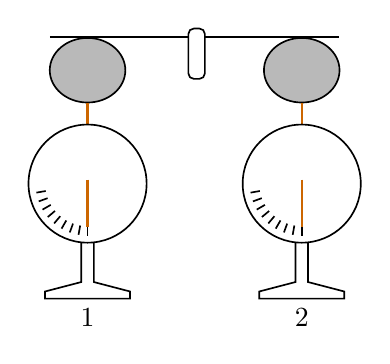
\begin{tikzpicture}[>=stealth,line width=.6pt]

\foreach \x/\n in {0/1,2.72/2}{
 \draw[fill=gray!55] (\x,1.82) ellipse(.48 and .41);
 \draw[orange!80!black,thick] (\x,1.41)--(\x,1.13);
 \draw (\x,.38) circle(.75);
 \draw (\x-.08,-.37)--(\x-.08,-.87)--(\x-.54,-.99)--(\x-.54,-1.08)--(\x+.54,-1.08)--(\x+.54,-.99)--(\x+.08,-.87)--(\x+.08,-.37);
 \foreach \t in {190,200,...,270}{\draw(\x,.38)++(\t:.54)--++(\t:.12);}
 \node[below]at(\x,-1.08){$\n$};\draw[orange!80!black,thick](\x,.43)--++(0,-.6);}
\draw(-.48,2.24)--(3.19,2.24);
\draw[fill=white,rounded corners=.07cm](1.28,1.71)rectangle(1.49,2.35);

\end{tikzpicture}\end{center}

Рис. $1$


\begin{center}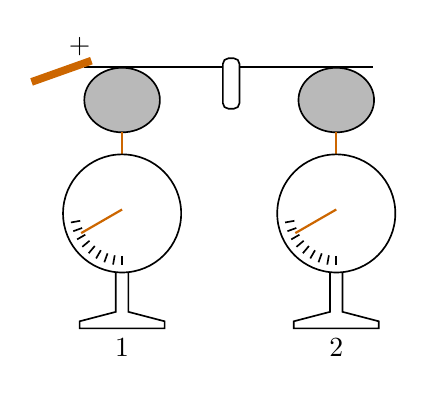
\begin{tikzpicture}[>=stealth,line width=.6pt]

\foreach \x/\n in {0/1,2.72/2}{
 \draw[fill=gray!55] (\x,1.82) ellipse(.48 and .41);
 \draw[orange!80!black,thick] (\x,1.41)--(\x,1.13);
 \draw (\x,.38) circle(.75);
 \draw (\x-.08,-.37)--(\x-.08,-.87)--(\x-.54,-.99)--(\x-.54,-1.08)--(\x+.54,-1.08)--(\x+.54,-.99)--(\x+.08,-.87)--(\x+.08,-.37);
 \foreach \t in {190,200,...,270}{\draw(\x,.38)++(\t:.54)--++(\t:.12);}
 \node[below]at(\x,-1.08){$\n$};\draw[orange!80!black,thick](\x,.43)--++(-.52,-.3);}
\draw(-.48,2.24)--(3.19,2.24);
\draw[fill=white,rounded corners=.07cm](1.28,1.71)rectangle(1.49,2.35);
\draw[orange!80!black,line width=2.8pt](-1.15,2.05)--(-.39,2.32);\node[above]at(-.54,2.26){$+$};
\end{tikzpicture}\end{center}

Рис. $2$

Ссылаясь на известные вам законы и явления, объясните, почему электрометры оказались заряженными, и определите знаки заряда каждого из электрометров после того, как палочку убрали.
}{
\smallskip\noindent\textbf{Решение}\par
Вокруг положительно заряженной палочки существует электрическое поле. Под его действием свободные электроны в проводнике (металлической палочке, металлических шарах) придут в движение, причем сила электрического действия будет направлена к заряженной палочке. В результате на шаре электрометра $1$ возникнет избыток электронов, а на шаре электрометра $2$ возникнет недостаток электронов. Данный процесс будет происходить до тех пор, пока потенциалы всех точек не станут равными. Таким образом, электрометр $1$ будет заряжен отрицательно, а электрометр $2$  — положительно.
Электрометры образуют изолированную систему, в которой выполняется закон сохранения электрического заряда. Так как до поднесения палочки система не имела заряда, то после на каждом шаре заряды будут равными по модулю и противоположными по знаку. После удаления стержня и палочки на каждом шаре останется индуцированный заряд.

Ответ: электрометр $1$ имеет отрицательный заряд, электрометр $2$  — положительный.
}

% Source 41562: https://phys-ege.sdamgia.ru/problem?id=41562
\BankTask{41562}{
На фотографии представлена электрическая цепь. Начертите принципиальную схему этой электрической цепи. Опираясь на законы постоянного тока, объясните, как должны измениться (уменьшиться, увеличиться или остаться прежними) показания идеальных амперметра и вольтметра при замыкании ключа. Учесть внутреннее сопротивление батарейки, а сопротивлением подводящих проводов и ключа пренебречь.

\begin{center}\begin{tikzpicture}[>=stealth,line width=.6pt]

\draw[fill=orange!30] (0,0)--(0,.88)--(.7,.62)--(.7,-.25)--cycle (.7,.62)--(1.1,.8)--(1.1,-.07)--(.7,-.25) (0,.88)--(.43,1.07)--(1.1,.8)--(.7,.62)--cycle;
\fill(.24,.84)circle(.045) (.67,.82)circle(.045);
\foreach \x/\y/\value/\sign in {.75/2.05/{03{,}2}/V,3.15/.9/{00{,}6}/A}{
 \draw[fill=orange!35](\x-.61,\y-.42)rectangle(\x+.61,\y+.91);
 \draw[fill=white](\x-.43,\y+.01)rectangle(\x+.43,\y+.81);
 \node at(\x,\y+.57){$\value$};\node at(\x,\y+.22){$\sign$};
 \fill(\x-.42,\y-.25)circle(.055) (\x+.42,\y-.25)circle(.055);}
\draw[fill=gray!25](5.02,1.31)rectangle(6.84,1.57);
\fill(5.17,1.52)circle(.04) (6.58,1.52)circle(.04);
\draw[orange!65!black,line width=1.4pt](5.17,1.52)--(5.97,1.98);
\foreach \x/\r in {5.22/3,6.82/2}{
 \draw[fill=gray!20](\x-.57,.15)rectangle(\x+.58,.42);
 \foreach \i in {-.36,-.27,...,.36}{\draw(\x+\i,.45)ellipse(.095 and .095);}
 \fill(\x-.48,.32)circle(.04) (\x+.49,.32)circle(.04);
 \node at(\x,-.05){$\r\,\text{Ом}$};}
\draw(.24,.84) to[out=125,in=-155](.33,1.8) (.67,.82) to[out=52,in=-1](1.17,1.8)
 (.67,.82)to[out=-17,in=177](2.73,.65) (3.57,.65)to[out=-14,in=155](4.74,.32)
 (4.74,.32)to[out=110,in=180](5.17,1.52) (5.71,.32)to[out=30,in=60](6.34,.32)
 (5.71,.32)to[out=137,in=-65](6.58,1.52) (7.31,.32)to[out=-10,in=-31](.24,.84);

\end{tikzpicture}\end{center}
}{
\smallskip\noindent\textbf{Решение}\par
Схема электрической цепи имеет следующий вид: 

\begin{center}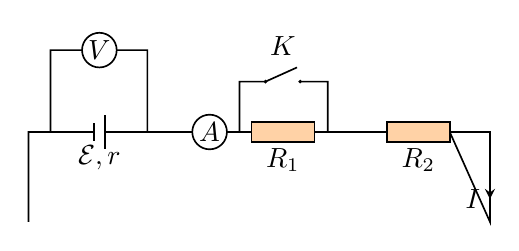
\begin{tikzpicture}[>=stealth,line width=.6pt]

\draw(0,0)--(0,1.14)--(.83,1.14) (.97,1.14)--(2.08,1.14) (2.52,1.14)--(2.83,1.14) (3.63,1.14)--(4.55,1.14) (5.35,1.14)--(5.86,1.14)--(5.86,0)--cycle
 (.28,1.14)--(.28,2.18)--(.68,2.18) (1.12,2.18)--(1.51,2.18)--(1.51,1.14)
 (2.68,1.14)--(2.68,1.78)--(3.01,1.78) (3.45,1.78)--(3.8,1.78)--(3.8,1.14);
\draw[->](5.86,.92)--(5.86,.29)node[left]{$I$};
\begin{scope}[shift={(0.9,1.14)},rotate=180]\draw(-.07,-.21)--(-.07,.21) (.07,-.11)--(.07,.11);\end{scope}\node[above right] at (1.02,1.14) {$$};\node[below] at(.9,1.1){$\mathcal E,r$};\draw (0.9,2.18)circle(.22) node {$V$};\draw (2.3,1.14)circle(.22) node {$A$};\begin{scope}[shift={(3.23,1.14)},rotate=0]\draw[fill=orange!35] (-.4,-.13) rectangle (.4,.13);\end{scope}\begin{scope}[shift={(4.95,1.14)},rotate=0]\draw[fill=orange!35] (-.4,-.13) rectangle (.4,.13);\end{scope}\node[below]at(3.23,1.06){$R_1$};\node[below]at(4.95,1.06){$R_2$};\begin{scope}[shift={(3.23,1.78)},rotate=0]\draw(-.22,0)--(.18,.18);\fill(-.22,0)circle(.025) (.22,0)circle(.025);\node[above]at(0,.2){$K$};\end{scope}
\end{tikzpicture}\end{center}

I  — сила тока в цепи.
При разомкнутом ключе ток будет проходить через резисторы R$_{1}$ и R$_{1}$, соединенные последовательно. Поэтому общее сопротивление цепи будет равно $R = R_1 + R_2.$
Амперметр измеряет общую силу тока в цепи, значение которой определяется законом Ома для полной цепи

\[I = \frac{\mathcal{E}}{R + r} ,\]

где $\mathcal{E}$  — ЭДС источника тока, r  — внутреннее сопротивление источника тока.
Исходя из закона Ома для участка цепи, содержащей последовательно соединенные резисторы, напряжение на внешней цепи, измеряемое вольтметром, U  =  IR. С учетом применения закона Ома для полной цепи данное напряжение равняется

\[U = \mathcal{E} - Ir.\]

Если замкнуть ключ, присоединенный параллельно к резистору R$_{1}$, то ток через данный резистор идти не будет. Поэтому общее сопротивление цепи станет равным R  =  R$_{2}$, а, следовательно, уменьшится. 
Из формулы закона Ома для полной цепи при уменьшении общего сопротивления сила тока в цепи увеличится. Напряжение соответственно формуле $U = \mathcal{E} - Ir.$ уменьшается.

Ответ: сила тока увеличивается, напряжение уменьшается.
}

% Source 19854: https://phys-ege.sdamgia.ru/problem?id=19854
\BankTask{19854}{
\begin{center}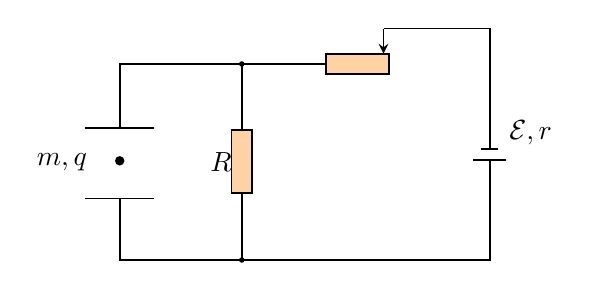
\begin{tikzpicture}[>=stealth,line width=.6pt]

\draw(0,1.17)--(0,1.98)--(2.62,1.98) (0,.27)--(0,-.51)--(4.7,-.51)--(4.7,.76)
 (4.7,.90)--(4.7,2.43)--(3.35,2.43);
\draw[->](3.35,2.43)--(3.35,2.11);
\draw(-.44,1.17)--(.44,1.17) (-.44,.27)--(.44,.27);
\draw(1.55,1.98)--(1.55,1.14) (1.55,.34)--(1.55,-.51);
\fill(0,.75)circle(.06) (1.55,1.98)circle(.035) (1.55,-.51)circle(.035);
\begin{scope}[shift={(3.02,1.98)},rotate=0]\draw[fill=orange!35] (-.4,-.13) rectangle (.4,.13);\end{scope}\begin{scope}[shift={(1.55,0.74)},rotate=90]\draw[fill=orange!35] (-.4,-.13) rectangle (.4,.13);\end{scope}\node[left] at (1.55,0.74) {$R$};\begin{scope}[shift={(4.7,0.83)},rotate=90]\draw(-.07,-.21)--(-.07,.21) (.07,-.11)--(.07,.11);\end{scope}\node[above right] at (4.82,0.83) {$\mathcal E,r$};\node[left]at(-.29,.73){$m,q$};
\end{tikzpicture}\end{center}
Две параллельные металлические пластины, расположенные горизонтально, подключены к электрической схеме, приведенной на рисунке. Между пластинами находится в равновесии маленькое заряженное тело массой m и зарядом q. Электростатическое поле между пластинами считать однородным. Опираясь на законы механики и электродинамики, объясните, как и в какую сторону начнет двигаться тело, если сдвинуть ползунок реостата влево.
}{
\smallskip\noindent\textbf{Решение}\par
\begin{center}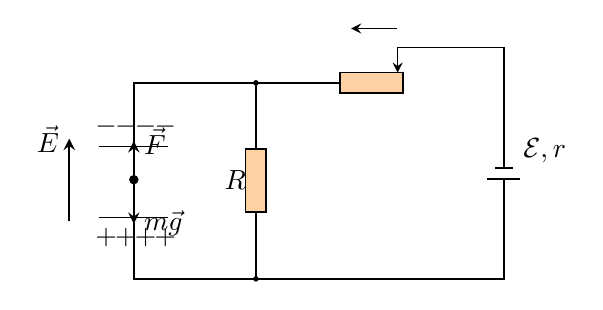
\begin{tikzpicture}[>=stealth,line width=.6pt]

\draw(0,1.17)--(0,1.98)--(2.62,1.98) (0,.27)--(0,-.51)--(4.7,-.51)--(4.7,.76)
 (4.7,.90)--(4.7,2.43)--(3.35,2.43);
\draw[->](3.35,2.43)--(3.35,2.11);
\draw(-.44,1.17)--(.44,1.17) (-.44,.27)--(.44,.27);
\draw(1.55,1.98)--(1.55,1.14) (1.55,.34)--(1.55,-.51);
\fill(0,.75)circle(.06) (1.55,1.98)circle(.035) (1.55,-.51)circle(.035);
\begin{scope}[shift={(3.02,1.98)},rotate=0]\draw[fill=orange!35] (-.4,-.13) rectangle (.4,.13);\end{scope}\begin{scope}[shift={(1.55,0.74)},rotate=90]\draw[fill=orange!35] (-.4,-.13) rectangle (.4,.13);\end{scope}\node[left] at (1.55,0.74) {$R$};\begin{scope}[shift={(4.7,0.83)},rotate=90]\draw(-.07,-.21)--(-.07,.21) (.07,-.11)--(.07,.11);\end{scope}\node[above right] at (4.82,0.83) {$\mathcal E,r$};
\foreach \x in {-.35,-.1,.15,.4}{\node at(\x,1.43){$-$};\node at(\x,.02){$+$};}
\draw[->,thick] (0,.75)--(0,.19)node[right]{$m\vec g$};
\draw[->,thick] (0,.75)--(0,1.24)node[right]{$\vec F$};
\draw[->,thick](-.82,.23)--(-.82,1.27)node[left]{$\vec E$};
\draw[->](3.34,2.67)--(2.76,2.67);

\end{tikzpicture}\end{center}
$1$.  Поскольку пластины подключены к источнику ЭДС, то между ними имеется разность потенциалов, в пространстве между ними создается однородное электростатическое поле. Согласно электрической схеме, нижняя пластина имеет положительный заряд, а верхняя  — отрицательный; следовательно, вектор напряженности поля направлен вертикально вверх. По условию задачи заряженное тело находится в равновесии; следовательно, сила тяжести скомпенсирована силой Кулона, направленной вертикально вверх. Отсюда делаем вывод, что тело имеет положительный заряд.
$2$.  Если сдвинуть ползунок реостата влево, то сопротивление реостата уменьшится. Поскольку реостат соединен с резистором R последовательно, то и общее сопротивление цепи также уменьшится. 
$3$.  Согласно закону Ома для полной цепи $\mathcal{E}=I ( R_{\,\text{цепи}} + r )$  — при уменьшении сопротивления внешней цепи сила тока в ней увеличится. Таким образом, по закону Ома для участка цепи цепи $U=IR$  — напряжение на резисторе R также увеличится. Поскольку пластины соединены с резистором R параллельно, то, соответственно, напряжение между ними увеличится. Следовательно, увеличится и напряженность поля между пластинами: $E=U/d.$
$4$.  Увеличение напряженности поля приведет к увеличению силы Кулона, действующей на тело: $F=qE.$ Равновесие нарушится, сила Кулона станет больше силы тяжести, и тело начнет двигаться вверх с ускорением.
}

% Source 29460: https://phys-ege.sdamgia.ru/problem?id=29460
\BankTask{29460}{
\begin{center}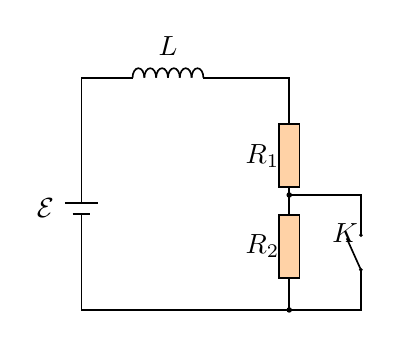
\begin{tikzpicture}[>=stealth,line width=.6pt]

\draw(0,.99)--(0,2.58)--(.65,2.58) (1.55,2.58)--(2.64,2.58)--(2.64,1.99)
 (2.64,1.19)--(2.64,.84) (2.64,.04)--(2.64,-.37)--(0,-.37)--(0,.85)
 (2.64,1.09)--(3.55,1.09)--(3.55,.58) (3.55,.14)--(3.55,-.37)--(2.64,-.37);
\fill(2.64,1.09)circle(.035) (2.64,-.37)circle(.035);
\begin{scope}[shift={(0,0.92)},rotate=-90]\draw(-.07,-.21)--(-.07,.21) (.07,-.11)--(.07,.11);\end{scope}\node[above right] at (0.12,0.92) {$$};\node[left]at(-.22,.92){$\mathcal E$};\begin{scope}[shift={(1.1,2.58)}]\foreach \x in {-.45,-.3,-.15,0,.15,.3}{\draw(\x,0)arc(180:0:.075 and .12);}\node[above] at (0,.15) {$L$};\end{scope}\begin{scope}[shift={(2.64,1.59)},rotate=90]\draw[fill=orange!35] (-.4,-.13) rectangle (.4,.13);\end{scope}\node[left] at (2.64,1.59) {$R_1$};\begin{scope}[shift={(2.64,0.44)},rotate=90]\draw[fill=orange!35] (-.4,-.13) rectangle (.4,.13);\end{scope}\node[left] at (2.64,0.44) {$R_2$};\begin{scope}[shift={(3.55,0.36)},rotate=90]\draw(-.22,0)--(.18,.18);\fill(-.22,0)circle(.025) (.22,0)circle(.025);\node[above]at(0,.2){$K$};\end{scope}
\end{tikzpicture}\end{center}
Катушка, обладающая индуктивностью L, соединена последовательно с источником постоянного тока с ЭДС $\mathcal{E}$ и резисторами R$_{1}$ и R$_{2}$, имеющими одинаковое сопротивление R$_{1}$ =  R$_{2}$  =  R, как показано на рисунке. В начальный момент ключ в цепи разомкнут. Как изменятся сила тока в цепи и напряжение на участке цепи, содержащем резистор R$_{1}$, после замыкания ключа? Ответ поясните, опираясь на законы электродинамики. Внутренним сопротивлением источника тока и сопротивлением катушки пренебречь.
}{
\smallskip\noindent\textbf{Решение}\par
$1$.  Сила тока определяется законом Ома для полной цепи: $IR_{\,\text{общ}}=\mathcal{E} + \mathcal E_{si},$ где I  — сила тока в цепи, $R_{\,\text{общ}}$  — сопротивление цепи, а $\mathcal E_{si}= - L \frac{\Delta I}{\Delta t}$  — ЭДС самоиндукции, возникающая только при изменении силы тока и препятствующая его изменению согласно правилу Ленца. 
$2$.  До замыкания ключа $R_{\,\text{общ}}=2R,$ сила тока через амперметр определяется законом Ома для замкнутой цепи: $I_1= \frac{\mathcal{E}}{2R} .$ 
$3$.  При замыкании ключа сопротивление цепи скачком уменьшается в $2$ раза, но ЭДС самоиндукции препятствует изменению силы тока через катушку. Поэтому сила тока через катушку при замыкании ключа не претерпевает скачка. 
$4$.  Постепенно ЭДС самоиндукции уменьшается до нуля, а сила тока через катушку плавно возрастает до стационарного значения: $I_2= \frac{\mathcal{E}}{R} ,$ в $2$ раза большего, чем начальное. 
$5$.  По закону Ома для участка цепи $U=IR_1$ увеличение тока через резистор R$_{1}$ приведет к увеличению напряжения на нем.
}

% Source 25381: https://phys-ege.sdamgia.ru/problem?id=25381
\BankTask{25381}{
\begin{center}\begin{tikzpicture}[>=stealth,line width=.6pt]

\draw(0,1)--(0,1.91) (0,2.29)--(0,2.75)--(4.51,2.75)--(4.51,2.3) (4.51,1.92)--(4.51,1.0)
 (4.51,.58)--(4.51,-.14)--(0,-.14)--(0,.58)
 (1.65,2.75)--(1.65,2.29) (1.65,1.49)--(1.65,1.25) (1.65,1.11)--(1.65,.53)
 (2.91,2.75)--(2.91,1.25) (2.91,1.11)--(2.91,.53);
\fill(1.65,.53)circle(.042) (2.91,.53)circle(.042) (2.28,.24)circle(.042);
\draw (2.28,-.14)--(2.28,.24);
\node[left]at(1.65,.45){$1$};\node[right]at(2.91,.45){$2$};
\draw(2.28,.24)--(1.65,.53);\begin{scope}[shift={(0,2.1)},rotate=-90]\draw(-.2,-.16)--(-.2,.16)--(.18,0)--cycle (.18,-.18)--(.18,.18);\end{scope}\node[left] at (0,2.3000000000000003) {$\text{Д1}$};\begin{scope}[shift={(4.51,2.11)},rotate=90]\draw(-.2,-.16)--(-.2,.16)--(.18,0)--cycle (.18,-.18)--(.18,.18);\end{scope}\node[right] at (4.51,2.31) {$\text{Д2}$};\begin{scope}[shift={(0,0.79)}]\draw(0,0)circle(.21) (-.14,-.14)--(.14,.14) (-.14,.14)--(.14,-.14);\node[left]at(-.23,0){Л1};\end{scope}\begin{scope}[shift={(4.51,0.79)}]\draw(0,0)circle(.21) (-.14,-.14)--(.14,.14) (-.14,.14)--(.14,-.14);\node[left]at(-.23,0){};\end{scope}\node[right]at(4.72,.79){Л2};\begin{scope}[shift={(1.65,1.89)},rotate=90]\draw[fill=orange!35] (-.4,-.13) rectangle (.4,.13);\end{scope}\node[left] at (1.65,1.89) {$R$};\begin{scope}[shift={(1.65,1.18)},rotate=-90]\draw(-.07,-.21)--(-.07,.21) (.07,-.11)--(.07,.11);\end{scope}\node[above right] at (1.77,1.18) {$$};\begin{scope}[shift={(2.91,1.18)},rotate=90]\draw(-.07,-.21)--(-.07,.21) (.07,-.11)--(.07,.11);\end{scope}\node[above right] at (3.0300000000000002,1.18) {$$};\node[left]at(1.46,1.18){$\mathcal E,r$};\node[right]at(3.09,1.18){$\mathcal E,r$};
\end{tikzpicture}\end{center}
На рисунке изображена схема электрической цепи, состоящей из двух одинаковых источников тока с ЭДС $\mathcal{E}$ и внутренним сопротивлением r, резистора сопротивлением R, двух одинаковых ламп Л1 и Л2, двух идеальных диодов Д1 и Д2 и ключа К. Опираясь на законы электродинамики, объясните, какие изменения произойдут в работе этой цепи, если перевести ключ К из положения $1$ в положение $2$. Сравните накал ламп в этих двух случаях.
}{
\smallskip\noindent\textbf{Решение}\par
При замыкании первого ключа ток не идет через правый источник тока. В этом случае цепь будет иметь вид, показанный на рис. $1$. Направление тока от плюса к минусу. При этом через диод Д1 ток идет в прямом направлении, а через диод Д2  — в обратном. Известно, что идеальный диод обладает малым сопротивлением при прохождении тока в прямом направлении и бесконечным сопротивлением при прохождении тока в обратном направлении. Тогда эквивалентная схема будет иметь вид, показанный на рис. $2$. 
При переводе ключа во второе положение, ток не будет идти через левый источник. Цепь будет иметь вид, показанный на рис. $3$. В этом случае ток через диод Д2 будет идти в прямом направлении, а через диод Д1  — в обратном. Тогда эквивалентная схема будет иметь вид, показанный на рис. $4$. 


\begin{center}\begin{tikzpicture}[>=stealth,line width=.6pt]

\draw(0,1)--(0,1.91) (0,2.29)--(0,2.75)--(4.51,2.75)--(4.51,2.3) (4.51,1.92)--(4.51,1.0)
 (4.51,.58)--(4.51,-.14)--(0,-.14)--(0,.58)
 (1.65,2.75)--(1.65,2.29) (1.65,1.49)--(1.65,1.25) (1.65,1.11)--(1.65,.53)
 (2.91,2.75)--(2.91,1.25) (2.91,1.11)--(2.91,.53);
\fill(1.65,.53)circle(.042) (2.91,.53)circle(.042) (2.28,.24)circle(.042);
\draw (2.28,-.14)--(2.28,.24);
\node[left]at(1.65,.45){$1$};\node[right]at(2.91,.45){$2$};
\draw(2.28,.24)--(1.65,.53);\draw[->](1.57,1.55)--(1.57,2.42);\draw[->](.85,2.57)--(.1,2.57);\draw[->](.18,1.7)--(.18,1.1);\draw[->](.66,.04)--(1.4,.04);\draw[->](3.3,2.57)--(4.37,2.57);\begin{scope}[shift={(0,2.1)},rotate=-90]\draw(-.2,-.16)--(-.2,.16)--(.18,0)--cycle (.18,-.18)--(.18,.18);\end{scope}\node[left] at (0,2.3000000000000003) {$\text{Д1}$};\begin{scope}[shift={(4.51,2.11)},rotate=90]\draw(-.2,-.16)--(-.2,.16)--(.18,0)--cycle (.18,-.18)--(.18,.18);\end{scope}\node[right] at (4.51,2.31) {$\text{Д2}$};\begin{scope}[shift={(0,0.79)}]\draw(0,0)circle(.21) (-.14,-.14)--(.14,.14) (-.14,.14)--(.14,-.14);\node[left]at(-.23,0){Л1};\end{scope}\begin{scope}[shift={(4.51,0.79)}]\draw(0,0)circle(.21) (-.14,-.14)--(.14,.14) (-.14,.14)--(.14,-.14);\node[left]at(-.23,0){};\end{scope}\node[right]at(4.72,.79){Л2};\begin{scope}[shift={(1.65,1.89)},rotate=90]\draw[fill=orange!35] (-.4,-.13) rectangle (.4,.13);\end{scope}\node[left] at (1.65,1.89) {$R$};\begin{scope}[shift={(1.65,1.18)},rotate=-90]\draw(-.07,-.21)--(-.07,.21) (.07,-.11)--(.07,.11);\end{scope}\node[above right] at (1.77,1.18) {$$};\begin{scope}[shift={(2.91,1.18)},rotate=90]\draw(-.07,-.21)--(-.07,.21) (.07,-.11)--(.07,.11);\end{scope}\node[above right] at (3.0300000000000002,1.18) {$$};\node[left]at(1.46,1.18){$\mathcal E,r$};\node[right]at(3.09,1.18){$\mathcal E,r$};
\end{tikzpicture}\end{center}

Рис. $1$ 


\begin{center}\begin{tikzpicture}[>=stealth,line width=.6pt]
\draw(0,1.02)--(0,2.4)--(2.61,2.4)--(2.61,1.86) (2.61,1.06)--(2.61,.74) (2.61,.6)--(2.61,-.18)--(0,-.18)--(0,.6);\begin{scope}[shift={(0,0.81)}]\draw(0,0)circle(.21) (-.14,-.14)--(.14,.14) (-.14,.14)--(.14,-.14);\node[left]at(-.23,0){Л1};\end{scope}\begin{scope}[shift={(2.61,1.46)},rotate=90]\draw[fill=orange!35] (-.4,-.13) rectangle (.4,.13);\end{scope}\node[left] at (2.61,1.46) {$R$};\begin{scope}[shift={(2.61,0.67)},rotate=-90]\draw(-.07,-.21)--(-.07,.21) (.07,-.11)--(.07,.11);\end{scope}\node[above right] at (2.73,0.67) {$\mathcal E,r$};
\end{tikzpicture}\end{center}

Рис. $2$ 


\begin{center}\begin{tikzpicture}[>=stealth,line width=.6pt]

\draw(0,1)--(0,1.91) (0,2.29)--(0,2.75)--(4.51,2.75)--(4.51,2.3) (4.51,1.92)--(4.51,1.0)
 (4.51,.58)--(4.51,-.14)--(0,-.14)--(0,.58)
 (1.65,2.75)--(1.65,2.29) (1.65,1.49)--(1.65,1.25) (1.65,1.11)--(1.65,.53)
 (2.91,2.75)--(2.91,1.25) (2.91,1.11)--(2.91,.53);
\fill(1.65,.53)circle(.042) (2.91,.53)circle(.042) (2.28,.24)circle(.042);
\draw (2.28,-.14)--(2.28,.24);
\node[left]at(1.65,.45){$1$};\node[right]at(2.91,.45){$2$};
\draw(2.28,.24)--(2.91,.53);\draw[->](3.8,2.57)--(3.2,2.57);\draw[->](3.08,1.0)--(3.08,.27);\draw[->](4.36,1.24)--(4.36,1.86);\draw[->](2.15,.04)--(1.5,.04);\draw[->](.16,1.22)--(.16,1.79);\begin{scope}[shift={(0,2.1)},rotate=-90]\draw(-.2,-.16)--(-.2,.16)--(.18,0)--cycle (.18,-.18)--(.18,.18);\end{scope}\node[left] at (0,2.3000000000000003) {$\text{Д1}$};\begin{scope}[shift={(4.51,2.11)},rotate=90]\draw(-.2,-.16)--(-.2,.16)--(.18,0)--cycle (.18,-.18)--(.18,.18);\end{scope}\node[right] at (4.51,2.31) {$\text{Д2}$};\begin{scope}[shift={(0,0.79)}]\draw(0,0)circle(.21) (-.14,-.14)--(.14,.14) (-.14,.14)--(.14,-.14);\node[left]at(-.23,0){Л1};\end{scope}\begin{scope}[shift={(4.51,0.79)}]\draw(0,0)circle(.21) (-.14,-.14)--(.14,.14) (-.14,.14)--(.14,-.14);\node[left]at(-.23,0){};\end{scope}\node[right]at(4.72,.79){Л2};\begin{scope}[shift={(1.65,1.89)},rotate=90]\draw[fill=orange!35] (-.4,-.13) rectangle (.4,.13);\end{scope}\node[left] at (1.65,1.89) {$R$};\begin{scope}[shift={(1.65,1.18)},rotate=-90]\draw(-.07,-.21)--(-.07,.21) (.07,-.11)--(.07,.11);\end{scope}\node[above right] at (1.77,1.18) {$$};\begin{scope}[shift={(2.91,1.18)},rotate=90]\draw(-.07,-.21)--(-.07,.21) (.07,-.11)--(.07,.11);\end{scope}\node[above right] at (3.0300000000000002,1.18) {$$};\node[left]at(1.46,1.18){$\mathcal E,r$};\node[right]at(3.09,1.18){$\mathcal E,r$};
\end{tikzpicture}\end{center}

Рис. $3$ 


\begin{center}\begin{tikzpicture}[>=stealth,line width=.6pt]
\draw(0,1.04)--(0,2.37)--(2.61,2.37)--(2.61,1.18) (2.61,.76)--(2.61,-.18)--(0,-.18)--(0,.9);\begin{scope}[shift={(2.61,0.97)}]\draw(0,0)circle(.21) (-.14,-.14)--(.14,.14) (-.14,.14)--(.14,-.14);\node[left]at(-.23,0){Л2};\end{scope}\begin{scope}[shift={(0,0.97)},rotate=90]\draw(-.07,-.21)--(-.07,.21) (.07,-.11)--(.07,.11);\end{scope}\node[above right] at (0.12,0.97) {$$};\node[left]at(-.24,.97){$\mathcal E,r$};
\end{tikzpicture}\end{center}

Рис. $4$ 

В первом случае в цепи лампа Л1 и резистор соединены последовательно. Их общее сопротивление равно $R + R_{\,\text{л}}.$ По закону Ома для полной цепи, сила тока $I_1= \frac{\mathcal{E}}{R + R_{\,\text{л}} + r} .$
Во втором случае в цепи будет только лампа Л2. По закону Ома для полной цепи сила тока $I_2= \frac{\mathcal{E}}{R_{\,\text{л}} + r} .$ Очевидно, что сопротивление уменьшилось, а сила тока увеличилась. Мощность тока в первом случае:

\[P_1=I_1 ^2 R_{\,\text{л}}= \frac{\mathcal E^2 R_{\text{л}}}{(R+R_{\text{л}}+r)^2} ,\]

во втором случае:

\[P_2=I_2 ^2 R_{\,\text{л}}= \frac{\mathcal E^2 R_{\text{л}}}{(R_{\text{л}}+r)^2} .\]

Из приведенных формул видно, что мощность тока увеличилась, следовательно, при переводе ключа из положения $1$ в положение $2$ накал одной из ламп увеличится, а другая лампа гореть не будет.

Ответ: накал горящей лампы увеличится.
}

% Source 16868: https://phys-ege.sdamgia.ru/problem?id=16868
\BankTask{16868}{
\begin{center}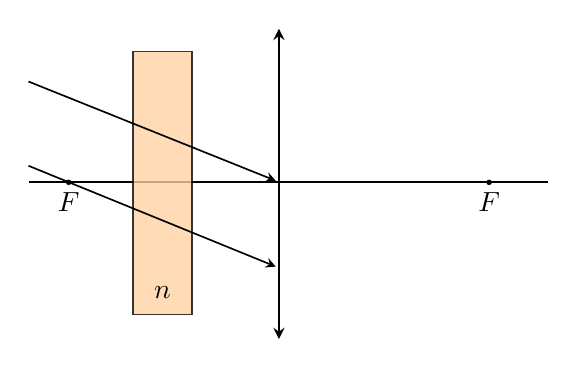
\begin{tikzpicture}[>=stealth,line width=.6pt]

\draw(-3.18,0)--(3.42,0);
\draw[<->,thick](0,-1.99)--(0,1.95);
\fill(-2.67,0)circle(.035) (2.67,0)circle(.035);
\node[below]at(-2.67,0){$F$};\node[below]at(2.67,0){$F$};
\draw[fill=orange!36,opacity=.78](-1.85,-1.68)rectangle(-1.10,1.66);\node at(-1.48,-1.4){$n$};\draw[->](-3.18,1.28)--(-.04,.02);\draw[->](-3.18,.21)--(-.04,-1.07);
\end{tikzpicture}\end{center}
На тонкую собирающую линзу от удаленного источника падает пучок параллельных лучей (см. рис.). Как изменится положение изображения источника, создаваемого линзой, если между линзой и ее фокусом поставить плоскопараллельную стеклянную пластинку с показателем преломления n (на рисунке положение пластинки отмечено пунктиром)? Ответ поясните, указав, какие физические закономерности Вы использовали. Сделайте рисунок, поясняющий ход лучей до и после установки плоскопараллельной стеклянной пластинки.
}{
\smallskip\noindent\textbf{Решение}\par
Построим изображение в линзе до и после установки плоскопараллельной пластинки. Для построения изображения пользуемся следующими соображениями. Луч, проходящий через центр линзы проходит непреломленным. Параллельный пучок света собирается в фокальной плоскости линзы.
После установки плоскопараллельной пластинки луч света будет преломляться внутри нее, но на выходе получим пучок света параллельный исходному. Поясним это соображение. По закону Снеллиуса оптические плотности сред n$_{1}$, n$_{2}$, угол падения $\alpha_{1}$, угол преломления $\alpha_{2}$, связаны соотношением: $n_1 \sin \alpha _1 = n_2 \sin \alpha _2.$ При выходе из пластины закон Снеллиуса также выполняется, получаем: $n_1 \sin \alpha _1 = n_2 \sin \alpha _2 = n_1 \sin \alpha _3.$ То есть синусы падающего и выходящего лучей равны, а значит, равны и углы под которыми, соответственно, падают и выходят эти лучи.


\begin{center}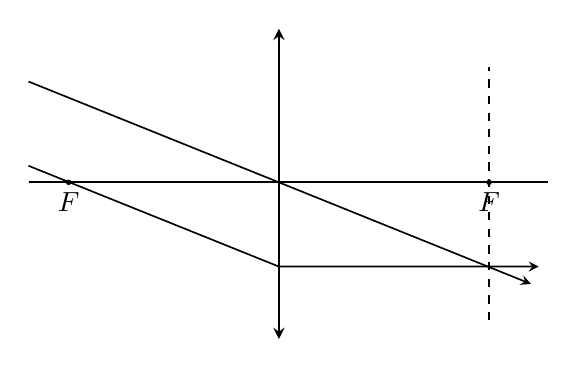
\begin{tikzpicture}[>=stealth,line width=.6pt]

\draw(-3.18,0)--(3.42,0);
\draw[<->,thick](0,-1.99)--(0,1.95);
\fill(-2.67,0)circle(.035) (2.67,0)circle(.035);
\node[below]at(-2.67,0){$F$};\node[below]at(2.67,0){$F$};
\draw[dashed](2.67,-1.75)--(2.67,1.47);\draw[->](-3.18,1.28)--(0,0)--(3.20,-1.29);\draw[->](-3.18,.21)--(0,-1.07)--(3.30,-1.07);
\end{tikzpicture}\end{center}



\begin{center}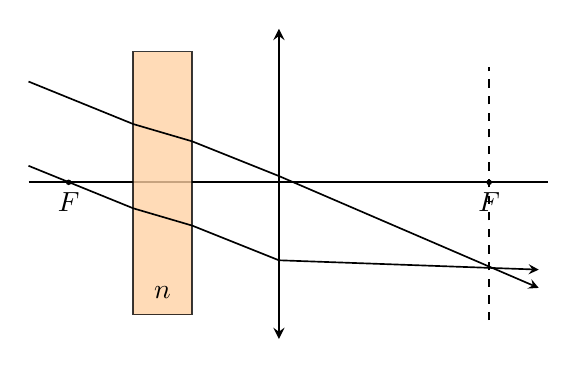
\begin{tikzpicture}[>=stealth,line width=.6pt]

\draw(-3.18,0)--(3.42,0);
\draw[<->,thick](0,-1.99)--(0,1.95);
\fill(-2.67,0)circle(.035) (2.67,0)circle(.035);
\node[below]at(-2.67,0){$F$};\node[below]at(2.67,0){$F$};
\draw[fill=orange!36,opacity=.78](-1.85,-1.68)rectangle(-1.10,1.66);\node at(-1.48,-1.4){$n$};\draw[dashed](2.67,-1.75)--(2.67,1.47);\draw[->](-3.18,1.28)--(-1.85,.74)--(-1.10,.52)--(0,.08)--(3.30,-1.341);\draw[->](-3.18,.21)--(-1.85,-.33)--(-1.10,-.55)--(0,-.99)--(3.30,-1.109);
\end{tikzpicture}\end{center}


Таким образом, получаем, что положение изображения источника после установки плоскопараллельной пластинки не изменится.
}

% Source 11810: https://phys-ege.sdamgia.ru/problem?id=11810
\BankTask{11810}{
\begin{center}\begin{tikzpicture}[>=stealth,line width=.6pt]

\draw[task grid,step=.46] (0,0) grid (3.22,2.76);
\draw[task axis] (0,0)--(3.39,0) node[right] {$U,\,\text{В}$};
\draw[task axis] (0,0)--(0,2.93) node[above left] {$P,\,\text{Вт}$};
\foreach \x in {0,...,6}{\node[below] at (.46*\x,0) {$\x$};}
\foreach \y in {1,...,4}{\node[left] at (0,.46*\y) {$\y$};}
\draw[task curve,orange!85!black,domain=0:2.76,samples=80] plot(\x,{(2.3/1.9044)*\x*(2.76-\x)});

\end{tikzpicture}\end{center}
Электрическая цепь состоит из батареи с ЭДС \ensuremath{\mathcal E} и внутренним сопротивлением r и подключенного к ней резистора нагрузки с сопротивлением R. При изменении сопротивления нагрузки изменяется напряжение на ней и мощность в нагрузке. На рисунке представлен график зависимости мощности, выделяющейся на нагрузке, от напряжения на ней. Используя известные Вам физические законы, объясните, почему данный график зависимости мощности от напряжения представляет собой параболу.
}{
\smallskip\noindent\textbf{Решение}\par
Мощность, выделяющаяся на нагрузке вычисляется по формуле: $P = UI = \frac{U ^2}{R} .$ Сила тока по закону Ома для полной цепи равна $I = \frac{\mathcal{E}}{r + R} .$ Напряжение на нагрузке вычисляется по формуле $U = IR = \frac{\mathcal{E} R}{r + R} ,$ откуда $R = \frac{Ur}{\mathcal{E} - U} .$ Таким образом, получаем: $P = \frac{U ^2}{Ur} \cdot ( \mathcal{E} - U ) = \frac{U ( \mathcal{E} - U )}{r} .$ Данная функция является квадратичной функцией от напряжения, ее график  — парабола.
}

% Source 25399: https://phys-ege.sdamgia.ru/problem?id=25399
\BankTask{25399}{
\begin{center}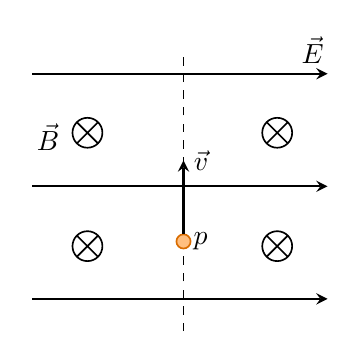
\begin{tikzpicture}[>=stealth,line width=.6pt]

\foreach \y in {-.9,.53,1.96}{\draw[->,thick](-1.68,\y)--(2.07,\y);}
\node[above]at(1.88,1.96){$\vec E$};
\foreach \x in {-.98,1.43}\foreach \y in {-.23,1.21}{\draw(\x,\y)circle(.19) (\x-.13,\y-.13)--(\x+.13,\y+.13) (\x-.13,\y+.13)--(\x+.13,\y-.13);}
\node[left]at(-1.21,1.15){$\vec B$};
\draw[dashed](.24,-1.31)--(.24,2.27);
\filldraw[fill=orange!50,draw=orange!85!black](.24,-.17)circle(.09) node[right]{$p$};
\draw[->,thick](.24,-.07)--(.24,.86)node[right]{$\vec v$};

\end{tikzpicture}\end{center}
В камере, из которой откачан воздух, создали электрическое поле напряженностью $\vec{E}$ и магнитное поле с индукцией $\vec{B}.$ Поля однородные, $\vec{E}\perp\vec{B}.$ В камеру влетает протон p, вектор скорости которого перпендикулярен $\overrightarrow{B}$ и $\overrightarrow{E}$ как показано на рисунке. Модули напряженности электрического поля и индукции магнитного поля таковы, что протон движется прямолинейно. Куда отклонится протон на начальном участке траектории, если его скорость уменьшить? Ответ поясните, указав, какие явления и закономерности Вы использовали для объяснения. Влиянием силы тяжести пренебречь.
}{
\smallskip\noindent\textbf{Решение}\par
На протон действует две силы: со стороны электрического поля $F_{\,\text{э}}=qE,$ направленная вправо, так как протон имеет положительный заряд; со стороны магнитного поля сила Лоренца $F_L=Bq v ,$ направленная влево по правилу левой руки. Протон движется равномерно, так как силы равны по модулю и противоположны, то есть равнодействующая этих сил равна $0$.
Если уменьшить скорость протона, то сила электрического поля не изменится, а сила Лоренца уменьшится. Тогда равнодействующая сила будет направлена вправо. Поскольку сила перпендикулярна скорости, то протон будет двигаться по криволинейной траектории, похожей на дугу окружности на начальном участке, отклоняясь вправо.
}

% Source 2914: https://phys-ege.sdamgia.ru/problem?id=2914
\BankTask{2914}{
\begin{center}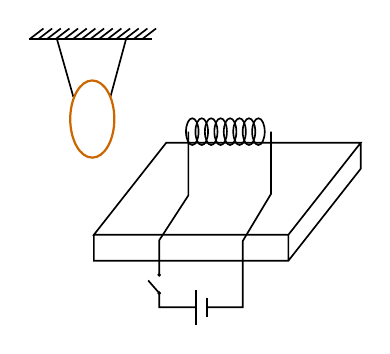
\begin{tikzpicture}[>=stealth,line width=.6pt]

\draw(-.65,2.88)--(.92,2.88);
\foreach \x in {-.63,-.52,...,.86}{\draw(\x,2.88)--++(.17,.13);}
\draw(-.29,2.88)--(-.08,2.14) (.59,2.88)--(.39,2.14);
\draw[orange!80!black,thick](.16,1.86)ellipse(.28 and .49);
\draw (.18,.39)--(2.65,.39)--(3.57,1.56)--(1.1,1.56)--cycle
 (.18,.39)--(.18,.06)--(2.65,.06)--(2.65,.39) (2.65,.06)--(3.57,1.23)--(3.57,1.56);
\draw(1.38,1.7)--(1.38,.89)--(1.01,.32)--(1.01,-.12) (2.43,1.7)--(2.43,.91)--(2.07,.31)--(2.07,-.53)--(1.62,-.53)
 (1.48,-.53)--(1.01,-.53)--(1.01,-.35);
\draw(1.01,-.35)--(.87,-.19);\fill(1.01,-.12)circle(.025) (1.01,-.35)circle(.025);
\foreach \x in {1.43,1.55,...,2.39}{\draw(\x,1.70)ellipse(.08 and .17);}
\draw(1.48,-.75)--(1.48,-.31) (1.62,-.65)--(1.62,-.41);

\end{tikzpicture}\end{center}
Замкнутое медное кольцо подвешено на длинных нитях вблизи катушки индуктивности, закрепленной на столе и подключенной к источнику постоянного тока (см. рис.). Первоначально электрическая цепь катушки разомкнута. Как будет двигаться кольцо при замыкании цепи? Ответ поясните, используя физические закономерности.
}{
\smallskip\noindent\textbf{Решение}\par
$1$.  При замыкании цепи катушки начинает изменяться поток вектора магнитной индукции через кольцо. По закону электромагнитной индукции в кольце возникает ЭДС индукции, появляется индукционный ток. В соответствии с правилом Ленца взаимодействие токов в кольце и в катушке приводит к тому, что кольцо отталкивается от катушки.
$2$.  Затем кольцо возвращается в исходное положение, так как ток в катушке достигает максимального значения, вследствие чего поток вектора магнитной индукции через кольцо становится постоянным. Индукционный ток в отсутствии ЭДС индукции затухает. Кольцо перестает отталкиваться от катушки.
$3$.  Индукционный ток в неподвижном кольце вблизи катушки с постоянным током равен нулю, магнитные свойства меди выражены слабо, поэтому, вернувшись в исходное положение равновесия, кольцо остается неподвижным.
}

% Source 29998: https://phys-ege.sdamgia.ru/problem?id=29998
\BankTask{29998}{
\begin{center}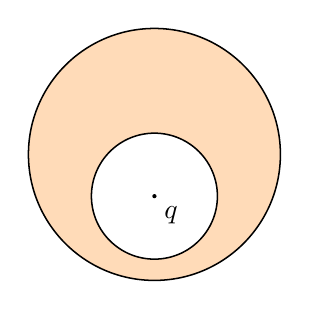
\begin{tikzpicture}[>=stealth,line width=.55pt]\draw[fill=orange!28](0,0)circle(1.6);\draw[fill=white](0,-.53)circle(.8);\fill(0,-.53)circle(.027)node[below right]{$q$};\end{tikzpicture}\end{center}В нижней половине незаряженного металлического шара располагается крупная шарообразная полость, заполненная воздухом. Шар находится в воздухе вдали от других предметов. В центр полости помещен положительный точечный заряд q > $0$ (см. рисунок). Нарисуйте картину линий напряженности электростатического поля внутри полости, внутри проводника и снаружи шара. Если поле отсутствует, напишите в данной области: $\vec{E} = 0.$ Если поле отлично от нуля, нарисуйте картину поля в данной области, используя восемь линий напряженности. Ответ поясните, указав, какие физические закономерности Вы использовали для объяснения.
}{
\smallskip\noindent\textbf{Решение}\par
\begin{center}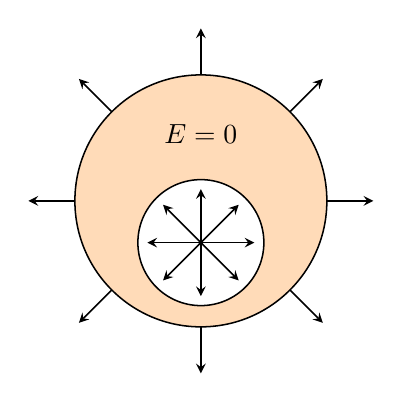
\begin{tikzpicture}[>=stealth,line width=.55pt]\draw[fill=orange!28](0,0)circle(1.6);\draw[fill=white](0,-.53)circle(.8);\node at(0,.85){$E=0$};\foreach \a in {0,45,...,315}{\draw[->](\a:1.6)--(\a:2.19);\draw[->](0,-.53)--++(\a:.68);}\fill(0,-.53)circle(.03);\end{tikzpicture}\end{center}$1$.  Приведен схематический рисунок картины линий напряженности: внутри полости  — семейство прямых лучей, исходящих из заряда и приходящих на поверхность полости по нормали; снаружи шара  — семейство прямых лучей, по нормали к ней и уходящих в бесконечность. 
$2$.  Внутри проводника  — электростатическое поле $\vec{E}=0.$ 
$3$.  Заряд q помещен в центр шарообразной полости, поэтому его электростатическое поле в полости обладает центральной симметрией и выглядит как поле уединенного точечного заряда $q > 0,$ находящегося в центре полости. Линии напряженности этого поля подходят по нормали к поверхности полости, где равномерно распределен отрицательный индуцированный заряд $- q < 0.$ 
$4$.  На наружной поверхности шара находится (в силу нейтральности шара в целом) положительный заряд $q > 0.$ Поскольку внутри проводника $\vec{E}=0,$ а снаружи окружающие предметы расположены далеко от шара, этот заряд распределен по поверхности шара равномерно. Его поле вне шара выглядит как поле уединенного точечного заряда q > $0$, расположенного в центре шара. Линии напряженности отходят от шара по нормали к его поверхности.
}

% Source 35341: https://phys-ege.sdamgia.ru/problem?id=35341
\BankTask{35341}{
\begin{center}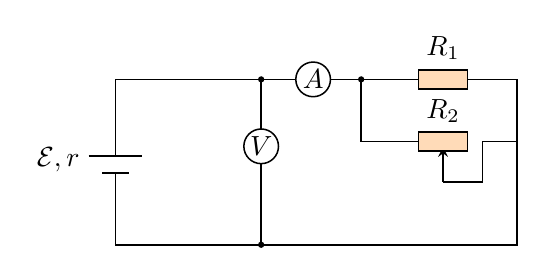
\begin{tikzpicture}[>=stealth,line width=.55pt]\draw(0,0)--(0,.91) (0,1.13)--(0,2.1)--(5.1,2.1)--(5.1,0)--(0,0);\draw(-.34,1.13)--(.34,1.13) (-.17,.91)--(.17,.91);\draw(1.85,0)--(1.85,2.1) (3.12,2.1)--(3.12,1.31)--(4.45,1.31);\fill(1.85,2.1)circle(.04) (1.85,0)circle(.04) (3.12,2.1)circle(.04);\draw[->](4.16,.8)--(4.16,1.24);\draw(4.16,.8)--(4.66,.8)--(4.66,1.31)--(5.1,1.31);\node[left]at(-.33,1.08){$\mathcal E,r$};\draw[fill=orange!28](3.85,1.98)rectangle(4.47,2.22);\node[above]at(4.16,2.22){$R_1$};\draw[fill=orange!28](3.85,1.19)rectangle(4.47,1.4300000000000002);\node[above]at(4.16,1.4300000000000002){$R_2$};\draw[fill=white](1.85,1.25)circle(.22)node{$V$};\draw[fill=white](2.51,2.1)circle(.22)node{$A$};\end{tikzpicture}\end{center}На рисунке показана принципиальная схема электрической цепи, состоящей из источника тока с отличным от нуля внутренним сопротивлением, резистора, реостата и измерительных приборов  — идеального амперметра и идеального вольтметра. Как будут изменяться показания приборов при перемещении движка реостата вправо? Ответ поясните, указав, какие физические закономерности Вы использовали для объяснения.
}{
\smallskip\noindent\textbf{Решение}\par
По условию задачи сопротивлением амперметра можно пренебречь, а сопротивление вольтметра бесконечно велико. При перемещении движка вправо сопротивление реостата R$_{2}$ увеличивается, что ведет к увеличению сопротивления R всей внешней цепи: $R= \frac{R_1 R_2}{R_1 + R_2} .$
В соответствии с законом Ома для полной цепи сила тока через амперметр уменьшается: $I= \frac{\mathcal{E}}{r + R}$ (знаменатель дроби растет, а числитель остается неизменным). Напряжение, измеряемое вольтметром, при этом растет: $U=I R=\mathcal{E} - I r.$

Ответ: напряжение, измеренное вольтметром, растет, а показания амперметра уменьшаются.
}

% Source 29732: https://phys-ege.sdamgia.ru/problem?id=29732
\BankTask{29732}{
Воспользовавшись оборудованием, представленным на левом рисунке, учитель собрал модель плоского конденсатора (см. средний рис.), зарядил нижнюю пластину положительным зарядом, а корпус электрометра заземлил. Соединенная с корпусом электрометра верхняя пластина конденсатора приобрела отрицательный заряд, равный по модулю заряду нижней пластины. После этого учитель сместил одну пластину относительно другой не изменяя расстояния между ними (см. правый рис.). Как изменились при этом показания электрометра (увеличились, уменьшились, остались прежними)? Ответ поясните, указав, какие явления и закономерности вы использовали для объяснения. Показания электрометра в данном опыте прямо пропорциональны разности потенциалов между пластинами конденсатора.

\begin{center}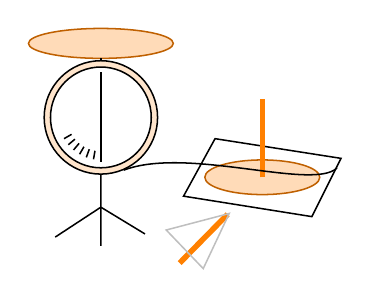
\begin{tikzpicture}[>=stealth,line width=.55pt]\draw[fill=orange!20](0,0)circle(.72);\draw[fill=white](0,0)circle(.64);\draw(0,-.72)--(0,-1.14)--(-.58,-1.52) (0,-1.14)--(.56,-1.48) (0,-1.14)--(0,-1.63);\foreach \a in {210,220,...,270}{\draw(\a:.43)--(\a:.54);}\draw(0,-.56)--(0,.58);\draw[thick](0,0)--(270:.56);\filldraw[fill=orange!28,draw=orange!75!black](0,.94)ellipse(.92 and .19);\draw(0,.75)--(0,.72);\begin{scope}[shift={(2.05,-.76)}]\draw(-1,-.24)--(.63,-.5)--(1,.24)--(-.6,.49)--cycle;\filldraw[fill=orange!28,draw=orange!75!black](0,0)ellipse(.73 and .22);\draw[orange,line width=2pt](0,0)--(0,1);\end{scope}\draw(.29,-.67) .. controls (1.1,-.36) and (2.7,-.94) .. (3,-.64);\draw[orange,line width=2pt](1,-1.85)--(1.61,-1.23);\draw[gray!50](.83,-1.43)--(1.63,-1.22)--(1.3,-1.92)--cycle;\end{tikzpicture}\end{center}

\begin{center}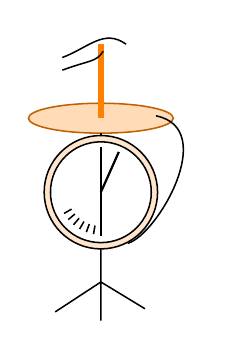
\begin{tikzpicture}[>=stealth,line width=.55pt]\draw[fill=orange!20](0,0)circle(.72);\draw[fill=white](0,0)circle(.64);\draw(0,-.72)--(0,-1.14)--(-.58,-1.52) (0,-1.14)--(.56,-1.48) (0,-1.14)--(0,-1.63);\foreach \a in {210,220,...,270}{\draw(\a:.43)--(\a:.54);}\draw(0,-.56)--(0,.58);\draw[thick](0,0)--(66:.56);\filldraw[fill=orange!28,draw=orange!75!black](0,.94)ellipse(.92 and .19);\draw(0,.75)--(0,.72);\draw[orange,line width=2pt](0,.94)--(0,1.88);\draw(.32,1.88)..controls(.04,2.08)and(-.15,1.84)..(-.49,1.71) (-.49,1.55)..controls(-.14,1.68)and(-.06,1.65)..(.03,1.79);\draw(.7,.97)..controls(1.5,.81)and(.72,-.54)..(.34,-.65);\end{tikzpicture}\end{center}

\begin{center}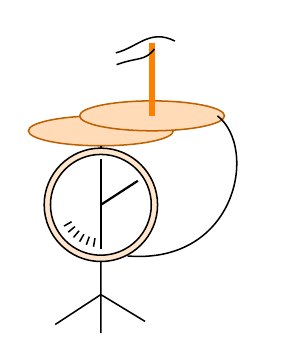
\begin{tikzpicture}[>=stealth,line width=.55pt]\draw[fill=orange!20](0,0)circle(.72);\draw[fill=white](0,0)circle(.64);\draw(0,-.72)--(0,-1.14)--(-.58,-1.52) (0,-1.14)--(.56,-1.48) (0,-1.14)--(0,-1.63);\foreach \a in {210,220,...,270}{\draw(\a:.43)--(\a:.54);}\draw(0,-.56)--(0,.58);\draw[thick](0,0)--(33:.56);\filldraw[fill=orange!28,draw=orange!75!black](0,.94)ellipse(.92 and .19);\draw(0,.75)--(0,.72);\filldraw[fill=orange!28,draw=orange!75!black](.65,1.13)ellipse(.92 and .19);\draw[orange,line width=2pt](.65,1.13)--(.65,2.05);\draw(.94,2.08)..controls(.62,2.24)and(.47,2)..(.19,1.93) (.2,1.78)..controls(.47,1.88)and(.56,1.82)..(.68,1.98);\draw(1.48,1.13)..controls(2,.73)and(1.73,-.76)..(.34,-.65);\end{tikzpicture}\end{center}
}{
\smallskip\noindent\textbf{Решение}\par
$1$.  При зарядке нижней пластины конденсатора стрежень и стрелка электрометра зарядятся одноименно с этой пластиной положительным зарядом. Соответственно, пластина, соединенная с корпусом получит отрицательный заряд. Данная система является замкнутой, поэтому в ней выполняется закон сохранения заряда. 
$2$.  При уменьшении общей площади пластин конденсатора уменьшится его емкость, исходя из формулы $C= \frac{\varepsilon \varepsilon_0 S}{d} .$ 
$3$.  Так как заряд на конденсаторе не изменился, его емкость уменьшилась, то разность потенциалов между его пластинами, исходя из формулы $C= \frac{q}{U} ,$ увеличилась. Соответственно, увеличилась разность потенциалов на электрометре. По условию угол отклонения стрелки электрометра пропорционален разности потенциалов. Следовательно, угол отклонения стрелки электрометра увеличился. 

Ответ: угол отклонения увеличится.
}

% Source 7159: https://phys-ege.sdamgia.ru/problem?id=7159
\BankTask{7159}{
\begin{center}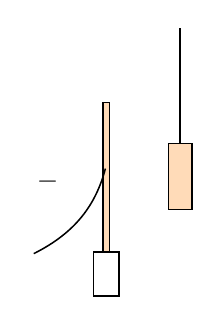
\begin{tikzpicture}[>=stealth,line width=.55pt]\draw(0,0)rectangle(.32,.56);\draw[fill=orange!28](.12,.56)rectangle(.2,2.46);\draw(1.1,3.4)--(1.1,1.94);\draw[fill=orange!28](.95,1.1)rectangle(1.25,1.94);\draw(-.76,.54)..controls(-.22,.81)and(.03,1.17)..(.15,1.62);\node[left]at(-.32,1.45){$-$};\end{tikzpicture}\end{center}Около небольшой металлической пластины, укрепленной на изолирующей подставке, подвесили на шелковой нити легкую металлическую незаряженную гильзу. Когда пластину подсоединили к клемме высоковольтного выпрямителя, подав на нее отрицательный заряд, гильза пришла в движение. Опишите движение гильзы и объясните его.
}{
\smallskip\noindent\textbf{Решение}\par
Под действием электрического поля пластины изменится распределение электронов в гильзе и произойдет ее электризация: та ее сторона, которая ближе к пластине, будет иметь положительный заряд, а противоположная сторона  — отрицательный.
Поскольку силы взаимодействия заряженных тел уменьшаются с ростом расстояния между ними, притяжение к пластине левой стороны гильзы будет сильнее отталкивания правой стороны гильзы, и гильза будет двигаться к пластине, пока не коснется ее.
В момент касания часть электронов перейдет с отрицательно заряженной пластины на гильзу, гильза приобретет отрицательный заряд и оттолкнется от одноименно заряженной пластины. Гильза отклонится вправо и зависнет в положении, в котором равнодействующая всех сил равна нулю.
}

% Source 29734: https://phys-ege.sdamgia.ru/problem?id=29734
\BankTask{29734}{
\begin{center}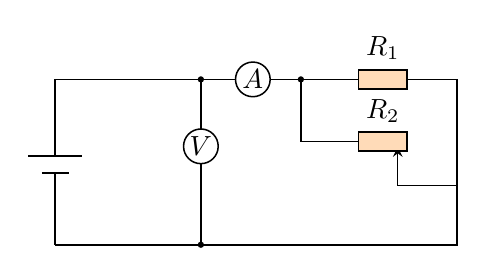
\begin{tikzpicture}[>=stealth,line width=.55pt]\draw(0,0)--(0,.91) (0,1.13)--(0,2.1)--(5.1,2.1)--(5.1,0)--(0,0);\draw(-.34,1.13)--(.34,1.13) (-.17,.91)--(.17,.91);\draw(1.85,0)--(1.85,2.1) (3.12,2.1)--(3.12,1.31)--(4.45,1.31);\fill(1.85,2.1)circle(.04) (1.85,0)circle(.04) (3.12,2.1)circle(.04);\draw[->](4.35,.75)--(4.35,1.24);\draw(4.35,.75)--(5.1,.75);\draw[fill=orange!28](3.85,1.98)rectangle(4.47,2.22);\node[above]at(4.16,2.22){$R_1$};\draw[fill=orange!28](3.85,1.19)rectangle(4.47,1.4300000000000002);\node[above]at(4.16,1.4300000000000002){$R_2$};\draw[fill=white](1.85,1.25)circle(.22)node{$V$};\draw[fill=white](2.51,2.1)circle(.22)node{$A$};\end{tikzpicture}\end{center} На рисунке изображена схема, содержащая источник тока с некоторым внутренним сопротивлением, резистор, реостат, амперметр и вольтметр. Как изменятся показания амперметра и вольтметра, если передвинуть ползунок реостата влево. Ответ поясните, указав, какие физические явления и закономерности Вы использовали для объяснения.
}{
\smallskip\noindent\textbf{Решение}\par
$1$.  При перемещении ползунка реостата влево происходит уменьшение длины проводника. Исходя из формулы для расчета сопротивления $R=\rho \frac{l}{S} ,$ делаем вывод, что сопротивление реостата $R_2$ уменьшается. 
$2$.  Реостат и резистор соединены между собой параллельно. Из формулы расчета общего сопротивления цепи $\frac{1}{R} = \frac{1}{R_1} + \frac{1}{R_2}$ следует, что общее сопротивление цепи также уменьшается. 
$3$.  По закону Ома для полной цепи $I= \frac{\mathcal{E}}{R + r}$ уменьшение общего сопротивления приведет к увеличению силы тока. Поскольку амперметр измеряет силу тока в неразветвленной части цепи, то его показания увеличатся. 
$4$.  Используя законы Ома для полной цепи и для участка цепи $I= \frac{U}{R} ,$ получаем, что $U=\mathcal{E} - I r.$ Увеличение силы тока приведет к уменьшению напряжения. Поскольку вольтметр измеряет напряжение на внешнем участке цепи, делаем вывод, что его показания уменьшаются. 

Ответ: показания амперметра увеличиваются, показания вольтметра уменьшаются.
}

% Source 9327: https://phys-ege.sdamgia.ru/problem?id=9327
\BankTask{9327}{
\begin{center}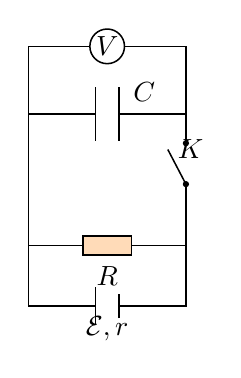
\begin{tikzpicture}[>=stealth,line width=.55pt]\draw(0,0)--(0,3.3)--(2,3.3)--(2,2.07) (2,1.55)--(2,0)--(1.15,0) (.85,0)--(0,0) (0,2.44)--(.85,2.44) (1.15,2.44)--(2,2.44) (0,.77)--(2,.77);\draw(.85,-.24)--(.85,.24) (1.15,-.15)--(1.15,.15) (.85,2.1)--(.85,2.78) (1.15,2.1)--(1.15,2.78);\fill(2,2.07)circle(.04) (2,1.55)circle(.04);\draw(2,1.55)--(1.77,1.99)node[right]{$K$};\node at(1.47,2.72){$C$};\node[below]at(1,0){$\mathcal E,r$};\draw[fill=white](1,3.3)circle(.22)node{$V$};\draw[fill=orange!28](0.69,0.65)rectangle(1.31,0.89);\node[above]at(1,0.89){$$};\node[below]at(1,.63){$R$};\end{tikzpicture}\end{center}Опираясь на законы физики, найдите показание идеального вольтметра в схеме, представленной на рисунке, до замыкания ключа К и опишите изменения его показаний после замыкания ключа К. Первоначально конденсатор не заряжен.
}{
\smallskip\noindent\textbf{Решение}\par
$1$.  Начальное показание вольтметра равно нулю, после замыкания ключа показания вольтметра будут увеличиваться, пока не достигнут максимального значения, которое не будет меняться со временем.
$2$.  Вольтметр соединен параллельно с конденсатором, поэтому его показания равны напряжению на конденсаторе. Вначале конденсатор не заряжен $( q_1=0 ) ,$ поэтому напряжение на нем $U_1= \frac{q_1}{C} =0,$ и показания вольтметра равны нулю.
$3$.  После замыкания конденсатор будет заряжаться, и, так как $U= \frac{q}{C} ,$ показания вольтметра будут увеличиваться. Когда конденсатор полностью зарядится, ток через него не течет, а течет только через резистор. Сила тока в цепи станет постоянной и согласно закону Ома для полной цепи $I= \frac{\varepsilon}{R + r} .$ Напряжение на конденсаторе и резисторе $U=IR$ и не будет меняться со временем. Поэтому показания вольтметра тоже перестанут изменяться.
}

% Source 7941: https://phys-ege.sdamgia.ru/problem?id=7941
\BankTask{7941}{
\begin{center}\begin{tikzpicture}[>=stealth,line width=.55pt]\draw(-3.9,0)--(3.48,0);\draw[<->,thick](0,-1.65)--(0,1.65)node[above left]{Л};\draw[->](-3.08,0)--(-3.08,.91)node[above]{$B$};\node[below]at(-3.08,0){$A$};\end{tikzpicture}\end{center}С помощью тонкой линзы на экране получают изображение объекта AB, расположенного параллельно ей. После чего линзу закрывают ободком из черного картона. Нарисуйте ход лучей и объясните, что произойдет с изображением на экране.
}{
\smallskip\noindent\textbf{Решение}\par
\begin{center}\begin{tikzpicture}[>=stealth,line width=.55pt]\draw(-3.9,0)--(3.48,0);\draw[<->,thick](0,-1.65)--(0,1.65)node[above left]{Л};\draw[->](-3.08,0)--(-3.08,.91)node[above]{$B$};\node[below]at(-3.08,0){$A$};\draw[->](2.42,0)--(2.42,-.71)node[below]{$B\prime$};\node[above]at(2.42,0){$A\prime$};\foreach \y in {-1.2,-.88,-.56,-.27,0,.28,.58,.91,1.2}{\draw[orange!85!black,line width=.35pt](-3.08,.91)--(0,\y)--(2.42,-.71);}\node[above]at(1.35,0){$F$};\node[left]at(-3.12,.46){$a$};\node[below]at(-1.48,0){$x$};\node[below]at(1.92,0){$y$};\node[right]at(2.49,-.38){$b$};\end{tikzpicture}\end{center}Изображение было получено на экране, значит, оно действительное, а объект AB расположен от линзы на расстоянии больше фокусного. Построим изображение A'B'. Луч, идущий параллельно главной оптической оси, после преломления в линзе проходит через фокус, а луч, прошедший через пересечение главной оптической оси и линзы, не преломляется. Пересечение лучей дает точку B'. Все прочие лучи, идущие от B и преломляющиеся в линзе, также проходят через точку B'. 
Запишем уравнение тонкой линзы:

\[\frac{1}{F} = \frac{1}{x} + \frac{1}{y} \Longleftrightarrow y= \frac{xF}{x - F} ,\]

где x  — расстояние от объекта до линзы, y  — расстояние от линзы до изображения, F  — фокусное расстояние линзы. Расстояние y не зависит от высоты объекта, значит, изображение A'B' перпендикулярно главной оптической оси. Из построения получаем, что изображение перевернутое.
\begin{center}\begin{tikzpicture}[>=stealth,line width=.55pt]\draw(-3.9,0)--(3.48,0);\draw[<->,thick](0,-1.65)--(0,1.65)node[above left]{Л};\draw[->](-3.08,0)--(-3.08,.91)node[above]{$B$};\node[below]at(-3.08,0){$A$};\draw[->](2.42,0)--(2.42,-.71)node[below]{$B\prime$};\node[above]at(2.42,0){$A\prime$};\foreach \y in {-.86,-.58,-.29,0,.29,.58,.86}{\draw[orange!85!black,line width=.35pt](-3.08,.91)--(0,\y)--(2.42,-.71);}\foreach \y in {-1.22,-1.04,1.04,1.22}{\draw[orange!85!black,line width=.35pt](-3.08,.91)--(0,\y);}\draw[orange!80!black,line width=3pt](-.04,.93)--(-.04,1.39) (-.04,-.93)--(-.04,-1.39);\end{tikzpicture}\end{center}Размер изображения можно найти из подобия треугольников:

\[\frac{a}{b} = \frac{x}{y} \Longleftrightarrow b= \frac{ay}{x} .\]

После того как линзу закрыли ободком, часть лучей стала поглощаться картоном. Ход непоглощенных лучей остался без изменения. Следовательно, изображение на экране останется на месте, только будет тусклее.
}

% Source 29730: https://phys-ege.sdamgia.ru/problem?id=29730
\BankTask{29730}{
\begin{center}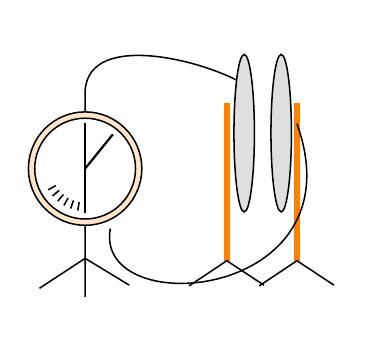
\begin{tikzpicture}[>=stealth,line width=.55pt]\draw[fill=orange!20](0,0)circle(.72);\draw[fill=white](0,0)circle(.64);\draw(0,-.72)--(0,-1.14)--(-.58,-1.52) (0,-1.14)--(.56,-1.48) (0,-1.14)--(0,-1.63);\foreach \a in {210,220,...,270}{\draw(\a:.43)--(\a:.54);}\draw(0,-.56)--(0,.58);\draw[thick](0,0)--(51:.56);\draw(0,.72)--(0,.99)..controls(.05,1.78)and(1.62,1.34)..(2.03,1.06);\draw[fill=gray!25](2.02,.45)ellipse(.13 and 1);\draw[fill=gray!25](2.49,.45)ellipse(.13 and 1);\foreach \x in {1.8,2.69}{\draw[orange,line width=2pt](\x,-1.17)--(\x,.83);\draw(\x,-1.17)--++(-.48,-.32) (\x,-1.17)--++(.47,-.31);}\draw(.32,-.76)..controls(.1,-1.95)and(3.5,-1.69)..(2.69,.57);\end{tikzpicture}\end{center} Две плоские пластины конденсатора, закрепленные на изолирующих штативах, расположили на небольшом расстоянии друг от друга и соединили одну пластину с заземленным корпусом, а другую  — со стержнем электрометра (см. рисунок). Затем пластину, соединенную со стержнем электрометра, зарядили. Объясните, опираясь на известные Вам законы, как изменяются показания электрометра при сближении пластин. Отклонение стрелки электрометра пропорционально разности потенциалов между пластинами. Емкость электрометра пренебрежимо мала.
}{
\smallskip\noindent\textbf{Решение}\par
$1$.  При зарядке левой пластины конденсатора стрежень и стрелка электрометра зарядятся одноименно с этой пластиной. Поскольку корпус электрометра заземлен, то на второй пластине конденсатора образуется заряд противоположного знака. Пластина со стержнем образуют замкнутую систему, поэтому в ней выполняется закон сохранения заряда. 
$2$.  При уменьшении расстояния между пластинами конденсатора увеличится его емкость, исходя из формулы $C= \frac{\varepsilon \varepsilon_0 S}{d} .$ 
$3$.  Так как заряд на конденсаторе не изменился, его емкость увеличилась, то разность потенциалов между его пластинами, исходя из формулы $C= \frac{q}{U} ,$ уменьшилась. Соответственно, уменьшилась разность потенциалов на электрометре. По условию угол отклонения стрелки электрометра пропорционален разности потенциалов. Следовательно, угол отклонения стрелки электрометра уменьшился. 

Ответ: угол отклонения уменьшится.
}

% Source 29880: https://phys-ege.sdamgia.ru/problem?id=29880
\BankTask{29880}{
\begin{center}\begin{tikzpicture}[>=stealth,line width=.55pt]\draw(0,-.48)arc(-140:-68:1.35) (-.3,-.13)arc(-140:-68:1);\draw[orange!85!black,->](1.41,-1.06)arc(-65:-159:1.15);\draw[->,orange!85!black](2.9,-1.07)--(1.6,-1.07);\draw(2.93,-1.34)rectangle(3.97,-.83)node[pos=.5]{И. Ч.};\draw(.1,-.58)--(.1,-1.87)--(5.03,-1.87)--(5.03,-.96) (-.18,-.31)--(5.03,-.31)--(5.03,-.63);\draw(5.03,-.7)circle(.07) (5.03,-.88)circle(.07);\node[right]at(5.12,-.8){$U$};\end{tikzpicture}\end{center}На рисунке показана схема устройства для предварительного отбора заряженных частиц для последующего детального исследования. Устройство представляет собой конденсатор, пластины которого изогнуты дугой радиусом $R.$ Перед попаданием в это пространство молекулы теряют один электрон. Во сколько раз надо изменить напряжение на обкладках конденсатора, чтобы сквозь него пролетали ионы, потерявшие два электрона? Влиянием силы тяжести пренебречь.
}{
\smallskip\noindent\textbf{Решение}\par
Центростремительное ускорение иона в конденсаторе $a= \frac{v ^2}{R}$ задается силой $F=qE= \frac{qU}{d}$ действия электрического поля, так что $\frac{qU}{d} =m \frac{v ^2}{R}$ (здесь q, m и \ensuremath{\upsilon} — соответственно заряд, масса и скорость иона; U  — напряжение на обкладках конденсатора, d  — расстояние между пластинами).
Тогда данное выражение имеет вид для каждого случая: 

$\frac{m v ^2}{R} = \frac{qU_1}{d}$ и $\frac{m v ^2}{R} = \frac{2qU_2}{d}$

Из соотношения видно, что для отбора ионов, потерявших два электрона, напряжение нужно уменьшить в $2$ раза.

Ответ:уменьшить в $2$ раза.
}

% Source 33064: https://phys-ege.sdamgia.ru/problem?id=33064
\BankTask{33064}{
Три параллельных длинных прямых проводника $1$, $2$ и $3$ расположены на одинаковом расстоянии а друг от друга (см. рис. а и б). В каждом проводнике протекает электрический ток силой I. Токи во всех проводниках текут в одном направлении. Определите направление результирующей силы, действующей на проводник $1$ со стороны проводников $2$ и $3$. Сделайте рисунок, указав в области проводника $1$ векторы магнитной индукции полей, созданных проводниками $2$ и $3$, вектор магнитной индукции результирующего магнитного поля и вектор результирующей силы. Ответ поясните, опираясь на законы электродинамики.

\begin{center}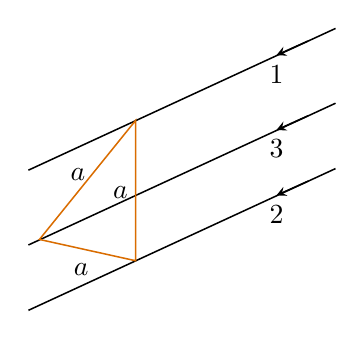
\begin{tikzpicture}[>=stealth,line width=.55pt]\draw(-.5,0)--(3.4,1.8) (-.5,.83)--(3.4,2.63) (-.5,1.78)--(3.4,3.58);\draw[orange!85!black](.86,.63)--(.86,2.41)--(-.36,.9)--cycle;\foreach \y/\i in {0/2,.83/3,1.78/1}{\draw[->](3.05,\y+1.64)--(2.65,\y+1.46)node[below]{$\i$};}\node at(.67,1.49){$a$};\node at(.13,1.73){$a$};\node at(.17,.52){$a$};\end{tikzpicture}\end{center}
Рис. а)

\begin{center}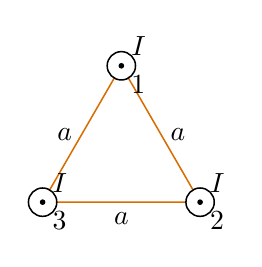
\begin{tikzpicture}[>=stealth,line width=.55pt]\draw[orange!85!black](0,0)--(2,0)--(1,1.732)--cycle;\foreach \x/\y/\i in {0/0/3,2/0/2,1/1.732/1}{\draw[fill=white](\x,\y)circle(.18);\fill(\x,\y)circle(.036);\node[below right]at(\x,\y){$\i$};\node[above right]at(\x,\y){$I$};}\node[below]at(1,0){$a$};\node[left]at(.5,.86){$a$};\node[right]at(1.5,.86){$a$};\end{tikzpicture}\end{center}
Рис. б)
}{
\smallskip\noindent\textbf{Решение}\par
На проводник $1$ со стороны проводников $2$ и $3$ действует результирующая сила, направленная вниз (см. рис.).
\begin{center}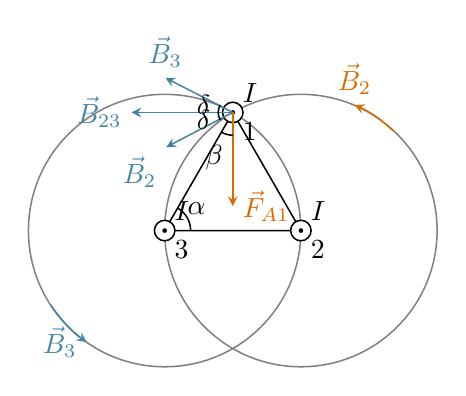
\begin{tikzpicture}[>=stealth,line width=.55pt]\draw[gray](0,0)circle(1.73) (1.73,0)circle(1.73);\draw(0,0)--(.865,1.5)--(1.73,0)--cycle;\foreach \x/\y/\i in {0/0/3,1.73/0/2,.865/1.5/1}{\draw[fill=white](\x,\y)circle(.13);\fill(\x,\y)circle(.03);\node[below right]at(\x,\y){$\i$};\node[above right]at(\x,\y){$I$};}\draw[->,cyan!60!black](.865,1.5)--(.01,1.94)node[above]{$\vec B_3$};\draw[->,cyan!60!black](.865,1.5)--(.02,1.06)node[below left]{$\vec B_2$};\draw[->,cyan!60!black](.865,1.5)--(-.42,1.5)node[left]{$\vec B_{23}$};\draw[->,orange!85!black](.865,1.5)--(.865,.31)node[right]{$\vec F_{A1}$};\draw[->,orange!85!black](2.91,1.26)arc(46:66:1.73)node[above]{$\vec B_2$};\draw[->,cyan!60!black](-1.45,-.94)arc(213:235:1.73)node[left]{$\vec B_3$};\draw(.68,1.5)arc(180:211:.185)node[left]{$\delta$};\draw(.68,1.5)arc(180:149:.185)node[left]{$\delta$};\draw(.33,0)arc(0:60:.33)node[right]{$\alpha$};\draw(.72,1.25)arc(240:270:.29)node[below left]{$\beta$};\end{tikzpicture}\end{center}
Вокруг проводников $2$ и $3$ возникает магнитное поле, линии индукции которого являются окружностями. Направление линий индукции магнитного поля определяется правилом буравчика. Вектор магнитной индукции результирующего поля в области проводника $1$ определяется принципом суперпозиции полей $\vec{B}_23=\vec{B}_2 + \vec{B}_3, \,\text{где}$ $\vec{B}_2$ и $\vec{B}_3$ − векторы индукции магнитных полей, созданных проводниками $2$ и Поскольку проводник $1$ находится на одинаковом расстоянии a от каждого из проводников $2$ и $3$, по проводникам протекают токи одинаковой силы, то $|\vec{B}_2|=|\vec{B}_3|=B.$
Из геометрических построений видно, что угол между векторами $\vec{B}_2$ и $\vec{B}_3$ составляет $60$°, значит, $\,\text{дельта} =30 ^\circ .$ Следовательно, вектор магнитной индукции $\vec{B}_23$ направлен горизонтально влево. Со стороны результирующего поля на проводник $1\,\text{с}$ током действует сила Ампера F$_{A1}$, направление которой определяется правилом левой руки. Таким образом, результирующая сила, действующая на проводник $1$ со стороны проводников $2$ и $3$, направлена вертикально вниз.

Ответ: на проводник $1$ со стороны проводников $2$ и $3$ действует результирующая сила, направленная вниз.
}

% Source 38951: https://phys-ege.sdamgia.ru/problem?id=38951
\BankTask{38951}{
Три одинаковых резистора и два одинаковых идеальных диода включены в электрическую цепь, показанную на рисунке, и подключены к аккумулятору в точках В и С. Показания амперметра равны $2\,\text{А}$. Определите силу тока через амперметр при смене полярности подключения аккумулятора. Нарисуйте эквивалентные электрические схемы для двух случаев подключения аккумулятора. Опираясь на законы электродинамики, поясните свой ответ. Сопротивлением амперметра и внутренним сопротивлением аккумулятора пренебречь.
\begin{center}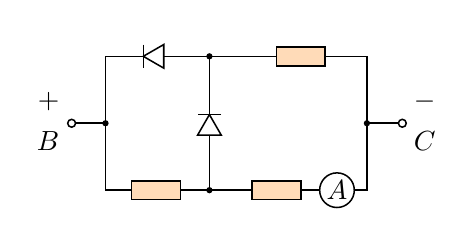
\begin{tikzpicture}[>=stealth,line width=.55pt]\draw(.5,.85)--(.88,.85) (.88,0)--(.88,1.7)--(4.2,1.7)--(4.2,0)--(.88,0) (4.2,.85)--(4.6,.85) (2.2,0)--(2.2,1.7);\fill(.88,.85)circle(.04) (4.2,.85)circle(.04) (2.2,0)circle(.04) (2.2,1.7)circle(.04);\draw(.45,.85)circle(.05) (4.65,.85)circle(.05);\node[left]at(.42,1.13){$+$};\node[left]at(.42,.63){$B$};\node[right]at(4.67,1.13){$-$};\node[right]at(4.67,.63){$C$};\begin{scope}[shift={(1.47,1.7)},rotate=180]\draw[fill=white](-.15,-.15)--(.11,0)--(-.15,.15)--cycle;\draw(.11,-.15)--(.11,.15);\end{scope}\begin{scope}[shift={(2.2,0.85)},rotate=90]\draw[fill=white](-.15,-.15)--(.11,0)--(-.15,.15)--cycle;\draw(.11,-.15)--(.11,.15);\end{scope}\draw[fill=orange!28](3.05,1.58)rectangle(3.67,1.8199999999999998);\node[above]at(3.36,1.8199999999999998){$$};\draw[fill=orange!28](1.21,-0.12)rectangle(1.83,0.12);\node[above]at(1.52,0.12){$$};\draw[fill=orange!28](2.7399999999999998,-0.12)rectangle(3.36,0.12);\node[above]at(3.05,0.12){$$};\draw[fill=white](3.82,0)circle(.22)node{$A$};\end{tikzpicture}\end{center}
}{
\smallskip\noindent\textbf{Решение}\par
При первом подключении цепи к источнику постоянного напряжения ток через верхний диод не проходит, через второй диод  — проходит, при этом точки, между которыми он находится, имеют равные потенциалы. Тогда эквивалентная схема имеет вид, изображенный на рис. $1$. Так как при параллельном соединении резисторы имеют одинаковое сопротивление, а амперметр идеальный, то через обе ветки идет ток, равный $2\,\text{А}$, а в неразветвленном участке цепи сила тока $I=I_1 + I_2=4\,\text{А}.$ Учитывая законы последовательного и параллельного соединения проводников, находим общее сопротивление цепи:   $R_{\,\text{общ}}= \frac{3R}{2} .$ Так как внутренним сопротивлением аккумулятора можно пренебречь, то напряжение на его клеммах равно по закону Ома $U=IR_{\,\text{общ}}=4 \cdot \frac{3R}{2} =6R.$
При изменении полярности подключения источника напряжения ток пройдет через оба диода, поэтому ток через левый резистор не пойдет. В этом случае получаем эквивалентную схему, изображенную на рис. $2$.
В цепи имеется два резистора, соединенные параллельно. Поэтому общее сопротивление цепи станет равным $R'_{\,\text{общ}}= \frac{R}{2} ,$ а общая сила тока $I'= \frac{U}{R'_{\,\text{общ}}} =12\,\text{А}.$ Так как обе ветви параллельно соединенных участков имеют одинаковое сопротивление, то ток через резистор и амперметр будет равен $I_A= \frac{I'}{2} = \frac{12}{2} =6\,\text{А}.$

\begin{center}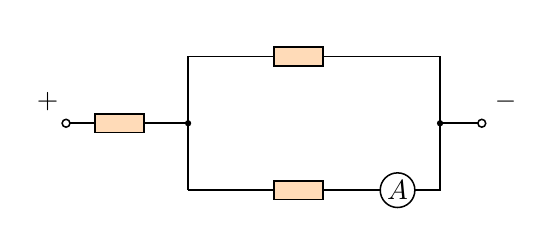
\begin{tikzpicture}[>=stealth,line width=.55pt]\draw(1,0)--(1,1.7)--(4.2,1.7)--(4.2,0)--(1,0);\fill(1,.85)circle(.04) (4.2,.85)circle(.04);\draw(4.2,.85)--(4.68,.85);\draw(4.73,.85)circle(.05);\draw(-.5,.85)--(1,.85);\draw(-.55,.85)circle(.05);\node[left]at(-.52,1.13){$+$};\node[right]at(4.77,1.13){$-$};\draw[fill=orange!28](-0.18,0.73)rectangle(0.44,0.97);\node[above]at(0.13,0.97){$$};\draw[fill=orange!28](2.09,1.58)rectangle(2.71,1.8199999999999998);\node[above]at(2.4,1.8199999999999998){$$};\draw[fill=orange!28](2.09,-0.12)rectangle(2.71,0.12);\node[above]at(2.4,0.12){$$};\draw[fill=white](3.66,0)circle(.22)node{$A$};\end{tikzpicture}\end{center}
Рис. $1$

\begin{center}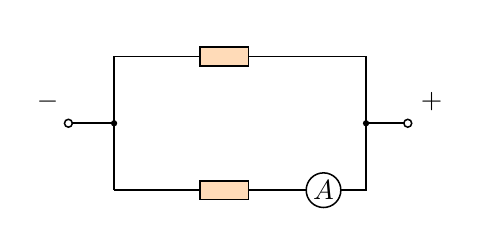
\begin{tikzpicture}[>=stealth,line width=.55pt]\draw(1,0)--(1,1.7)--(4.2,1.7)--(4.2,0)--(1,0);\fill(1,.85)circle(.04) (4.2,.85)circle(.04);\draw(4.2,.85)--(4.68,.85);\draw(4.73,.85)circle(.05);\draw(.47,.85)--(1,.85);\draw(.42,.85)circle(.05);\node[left]at(.42,1.13){$-$};\node[right]at(4.77,1.13){$+$};\draw[fill=orange!28](2.09,1.58)rectangle(2.71,1.8199999999999998);\node[above]at(2.4,1.8199999999999998){$$};\draw[fill=orange!28](2.09,-0.12)rectangle(2.71,0.12);\node[above]at(2.4,0.12){$$};\draw[fill=white](3.66,0)circle(.22)node{$A$};\end{tikzpicture}\end{center}
Рис. $2$

Ответ: сила тока через амперметр станет равной $6\,\text{А}$.
}

% Source 7873: https://phys-ege.sdamgia.ru/problem?id=7873
\BankTask{7873}{
Воспользовавшись оборудованием, представленным на рис. $1$, учитель собрал модель плоского конденсатора (рис. $2$), зарядил нижнюю пластину положительным зарядом, а корпус электрометра заземлил. Соединенная с корпусом электрометра верхняя пластина конденсатора приобрела отрицательный заряд, равный по модулю заряду нижней пластины. После этого учитель сместил одну пластину относительно другой не изменяя расстояния между ними (рис. $3$). Как изменились при этом показания электрометра (увеличились, уменьшились, остались прежними)? Ответ поясните, указав, какие явления и закономерности вы использовали для объяснения. Показания электрометра в данном опыте прямо пропорциональны разности потенциалов между пластинами конденсатора.

\begin{center}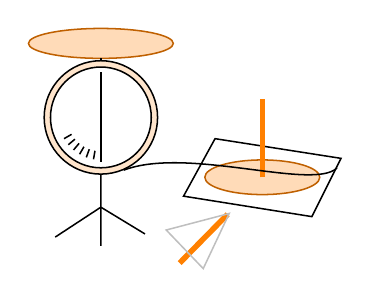
\begin{tikzpicture}[>=stealth,line width=.55pt]\draw[fill=orange!20](0,0)circle(.72);\draw[fill=white](0,0)circle(.64);\draw(0,-.72)--(0,-1.14)--(-.58,-1.52) (0,-1.14)--(.56,-1.48) (0,-1.14)--(0,-1.63);\foreach \a in {210,220,...,270}{\draw(\a:.43)--(\a:.54);}\draw(0,-.56)--(0,.58);\draw[thick](0,0)--(270:.56);\filldraw[fill=orange!28,draw=orange!75!black](0,.94)ellipse(.92 and .19);\draw(0,.75)--(0,.72);\begin{scope}[shift={(2.05,-.76)}]\draw(-1,-.24)--(.63,-.5)--(1,.24)--(-.6,.49)--cycle;\filldraw[fill=orange!28,draw=orange!75!black](0,0)ellipse(.73 and .22);\draw[orange,line width=2pt](0,0)--(0,1);\end{scope}\draw(.29,-.67) .. controls (1.1,-.36) and (2.7,-.94) .. (3,-.64);\draw[orange,line width=2pt](1,-1.85)--(1.61,-1.23);\draw[gray!50](.83,-1.43)--(1.63,-1.22)--(1.3,-1.92)--cycle;\end{tikzpicture}\end{center}
Рис. $1$

\begin{center}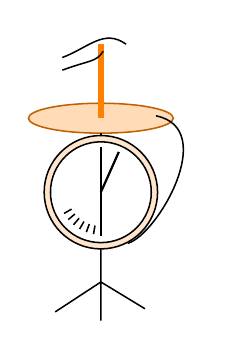
\begin{tikzpicture}[>=stealth,line width=.55pt]\draw[fill=orange!20](0,0)circle(.72);\draw[fill=white](0,0)circle(.64);\draw(0,-.72)--(0,-1.14)--(-.58,-1.52) (0,-1.14)--(.56,-1.48) (0,-1.14)--(0,-1.63);\foreach \a in {210,220,...,270}{\draw(\a:.43)--(\a:.54);}\draw(0,-.56)--(0,.58);\draw[thick](0,0)--(66:.56);\filldraw[fill=orange!28,draw=orange!75!black](0,.94)ellipse(.92 and .19);\draw(0,.75)--(0,.72);\draw[orange,line width=2pt](0,.94)--(0,1.88);\draw(.32,1.88)..controls(.04,2.08)and(-.15,1.84)..(-.49,1.71) (-.49,1.55)..controls(-.14,1.68)and(-.06,1.65)..(.03,1.79);\draw(.7,.97)..controls(1.5,.81)and(.72,-.54)..(.34,-.65);\end{tikzpicture}\end{center}
Рис. $2$

\begin{center}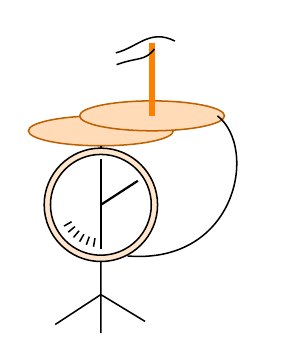
\begin{tikzpicture}[>=stealth,line width=.55pt]\draw[fill=orange!20](0,0)circle(.72);\draw[fill=white](0,0)circle(.64);\draw(0,-.72)--(0,-1.14)--(-.58,-1.52) (0,-1.14)--(.56,-1.48) (0,-1.14)--(0,-1.63);\foreach \a in {210,220,...,270}{\draw(\a:.43)--(\a:.54);}\draw(0,-.56)--(0,.58);\draw[thick](0,0)--(33:.56);\filldraw[fill=orange!28,draw=orange!75!black](0,.94)ellipse(.92 and .19);\draw(0,.75)--(0,.72);\filldraw[fill=orange!28,draw=orange!75!black](.65,1.13)ellipse(.92 and .19);\draw[orange,line width=2pt](.65,1.13)--(.65,2.05);\draw(.94,2.08)..controls(.62,2.24)and(.47,2)..(.19,1.93) (.2,1.78)..controls(.47,1.88)and(.56,1.82)..(.68,1.98);\draw(1.48,1.13)..controls(2,.73)and(1.73,-.76)..(.34,-.65);\end{tikzpicture}\end{center}
Рис. $3$
}{
\smallskip\noindent\textbf{Решение}\par
Стрелка и стержень, соединенные с пластиной, но изолированные от корпуса электрометра, заряжаются положительно, в результате взаимодействия стрелка отклоняется на некоторый угол.
Нижняя пластина создает вокруг себя электрическое поле, под действием которого в верхней пластине и металлическом корпусе электрометра происходит перераспределение зарядов, которое длится до тех пор, пока поверхности пластин не станут эквипотенциальными. В результате перераспределения зарядов верхняя пластинка заряжается отрицательно. Таким образом, заряды пластин становятся одинаковыми по модулю, но противоположными по знаку.
Система из двух заряженных пластин образует конденсатор емкостью $C = \frac{\,\text{эпсилон} \,\text{эпсилон} _0S}{d} .$ Поскольку расстояние между пластинами d и диэлектрическая проницаемость воздуха $\,\text{эпсилон}$ не изменились, а перекрываемая площадь пластин S уменьшилась, то и емкость конденсатора уменьшилась.
С другой стороны емкость конденсатора равна $C= \frac{q}{U} .$ Поскольку заряд на пластинах конденсатора остается постоянным, емкость уменьшается, то разность потенциалов между обкладками конденсатора увеличивается.
По условию задачи разность потенциалов пропорциональна показаниям электрометра, то при увеличении напряжения увеличивается угол отклонения стрелки. Показания электрометра увеличились.
}

% Source 2928: https://phys-ege.sdamgia.ru/problem?id=2928
\BankTask{2928}{
На рисунке приведена электрическая цепь, состоящая из гальванического элемента, реостата, трансформатора, амперметра и вольтметра.
\begin{center}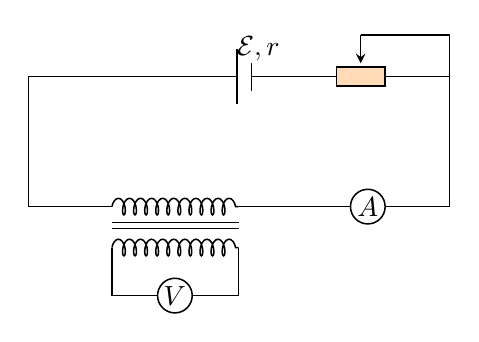
\begin{tikzpicture}[>=stealth,line width=.55pt]\draw(0,0)--(0,1.65)--(2.65,1.65) (2.83,1.65)--(5.35,1.65)--(5.35,0)--(2.67,0) (1.06,0)--(0,0);\draw(2.65,1.3)--(2.65,2) (2.83,1.47)--(2.83,1.83);\node[above]at(2.92,1.72){$\mathcal E,r$};\draw[->](4.22,2.18)--(4.22,1.82);\draw(4.22,2.18)--(5.35,2.18)--(5.35,1.65);\draw[decorate,decoration={coil,aspect=.45,amplitude=3pt,segment length=4pt}](1.06,0)--(2.67,0);\draw(1.06,-.2)--(2.67,-.2) (1.06,-.28)--(2.67,-.28);\draw[decorate,decoration={coil,aspect=.45,amplitude=3pt,segment length=4pt}](1.06,-.52)--(2.67,-.52);\draw(1.06,-.52)--(1.06,-1.13)--(2.67,-1.13)--(2.67,-.52);\draw[fill=orange!28](3.9099999999999997,1.5299999999999998)rectangle(4.529999999999999,1.77);\node[above]at(4.22,1.77){$$};\draw[fill=white](4.31,0)circle(.22)node{$A$};\draw[fill=white](1.86,-1.13)circle(.22)node{$V$};\end{tikzpicture}\end{center}
В начальный момент времени ползунок реостата установлен посередине и неподвижен. Опираясь на законы электродинамики, объясните, как будут изменяться показания приборов в процессе перемещения ползунка реостата вправо. ЭДС самоиндукции пренебречь по сравнению с $\mathcal E.$
}{
\smallskip\noindent\textbf{Решение}\par
$1$.  Во время перемещения движка реостата показания амперметра будут плавно уменьшаться, а вольтметр будет регистрировать напряжение на концах вторичной обмотки. Примечание: для полного ответа не требуется объяснения показаний приборов в крайнем правом положении. (Когда движок придет в крайнее правое положение и движение его прекратится, амперметр будет показывать постоянную силу тока в цепи, а напряжение, измеряемое вольтметром, окажется равным нулю.)
$2$.  При перемещении ползунка вправо сопротивление цепи увеличивается, а сила тока уменьшается в соответствии с законом Ома для полной цепи: $I= \frac{\mathcal E}{R + r} ,$ где R  — сопротивление внешней цепи.
Изменение тока, текущего по первичной обмотке трансформатора, вызывает изменение индукции магнитного поля, создаваемого этой обмоткой. Это приводит к изменению магнитного потока через вторичную обмотку трансформатора. В соответствии с законом индукции Фарадея возникает ЭДС индукции $\mathcal E = - \frac{\Delta \Phi}{\Delta t}$ во вторичной обмотке, а следовательно, напряжение U  на ее концах, регистрируемое вольтметром.
}

% Source 8554: https://phys-ege.sdamgia.ru/problem?id=8554
\BankTask{8554}{
\begin{center}\begin{tikzpicture}[>=stealth,line width=.55pt]\draw(0,2.1)--(-.55,1.95)--(-.55,.42)--(0,.19)--(.53,.42)--(.53,1.95)--(0,2.1);\draw(0,2.1)..controls(1.65,2.05)and(2.26,1.53)..(2.2,1.2)..controls(2.02,.55)and(1.96,.88)..(2.17,1.24)..controls(2.5,1.73)and(2.5,.98)..(2.24,.73)..controls(1.55,.27)and(.64,.19)..(0,.19);\foreach \x/\i in {-.55/1,.53/2}{\draw[fill=white](\x,1.59)circle(.19);\draw(\x-.13,1.46)--(\x+.13,1.72) (\x-.13,1.72)--(\x+.13,1.46);\node[left]at(\x-.19,1.57){$\i$};}\node[above]at(0,2.1){А};\node[below]at(0,.19){Б};\draw[->](.5,2.9)--(1.27,2.9);\draw[<-](.5,3.19)--(1.27,3.19);\draw(.98,3.05)--(1.16,3.33) (1.16,3.05)--(.98,3.33);\node[left]at(.35,3.02){$I$};\draw(.5,2.52)--(1.27,2.52);\draw[fill=cyan!25](2.9,.9)rectangle(3.55,1.48)node[pos=.5]{$N$};\draw[fill=red!25](3.55,.9)rectangle(4.2,1.48)node[pos=.5]{$S$};\draw[->,orange!85!black](4.08,.64)--(3.02,.64);\begin{scope}[shift={(-0.55,0.94)},rotate=-90]\draw[fill=white](-.15,-.15)--(.11,0)--(-.15,.15)--cycle;\draw(.11,-.15)--(.11,.15);\end{scope}\begin{scope}[shift={(0.53,0.94)},rotate=90]\draw[fill=white](-.15,-.15)--(.11,0)--(-.15,.15)--cycle;\draw(.11,-.15)--(.11,.15);\end{scope}\begin{scope}[shift={(0.97,2.52)},rotate=0]\draw[fill=white](-.15,-.15)--(.11,0)--(-.15,.15)--cycle;\draw(.11,-.15)--(.11,.15);\end{scope}\end{tikzpicture}\end{center}Электрическая цепь состоит из двух лампочек, двух диодов и витка провода, соединенных как показано на рисунке. (Диод пропускает ток только в одном направлении, как показано в верхней части рисунка.) Какая из лампочек загорится, если к витку приближать северный полюс магнита? Ответ объясните, указав, какие явления и закономерности Вы использовали при объяснении.
}{
\smallskip\noindent\textbf{Решение}\par
$1$.  Загорится лампочка $2$.
$2$.  При приближении магнита к витку будет меняться магнитный поток сквозь виток, и в витке возникнет индукционный ток. Согласно правилу Ленца магнитное поле этого тока должно препятствовать движению магнита, поэтому выходящие из витка линии индукции этого поля будут направлены в сторону магнита. Для создания такого поля, согласно правилу «буравчика», индукционный ток в цепи, содержащей виток, должен быть направлен по часовой стрелке (если смотреть слева), а в цепи ламп  — от Б к А. Ток такого направления пропускает только диод на участке цепи лампочки $2$, она и будет гореть.
}

% Source 4963: https://phys-ege.sdamgia.ru/problem?id=4963
\BankTask{4963}{
\begin{center}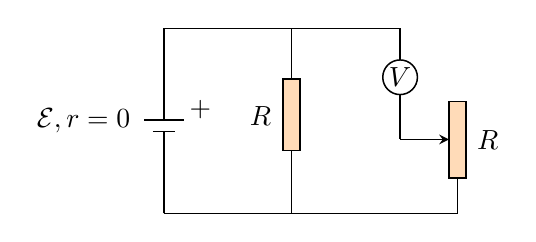
\begin{tikzpicture}[>=stealth,line width=.55pt]\draw(0,0)--(0,1.04) (0,1.19)--(0,2.35)--(3,2.35)--(3,.94) (0,0)--(3.73,0)--(3.73,1.42) (1.62,0)--(1.62,2.35);\draw(-.25,1.19)--(.25,1.19) (-.14,1.04)--(.14,1.04);\draw[->](3,.94)--(3.62,.94);\draw[fill=orange!28](1.51,.8)rectangle(1.73,1.71) (3.62,.45)rectangle(3.84,1.42);\node[left]at(-.3,1.18){$\mathcal E,r=0$};\node[right]at(.2,1.32){$+$};\node[left]at(1.49,1.24){$R$};\node[right]at(3.85,.93){$R$};\draw[fill=white](3,1.73)circle(.22)node{$V$};\end{tikzpicture}\end{center}В схеме на рисунке сопротивление резистора и полное сопротивление реостата равны R, ЭДС батарейки равна Е, ее внутреннее сопротивление ничтожно ($r = 0$). Как ведут себя (увеличиваются, уменьшаются, остаются постоянными) показания идеального вольтметра при перемещении движка реостата из крайнего верхнего в крайнее нижнее положение? Ответ поясните, указав, какие физические закономерности Вы использовали для объяснения.
}{
\smallskip\noindent\textbf{Решение}\par
Вольтметр подключают параллельно к тому участку, на котором нужно измерить напряжение. При этом, естественно, часть тока в цепи начинает течь через сам вольтметр. Тем самым вольтметр вносит возмущение в цепь и показывает напряжение, которое отличается от реального (когда вольтметра нет). Идеальным вольтметром называют прибор, который данной проблемой не страдает. То есть он имеет бесконечное собственное сопротивление. Действительно, рассмотрим положение ползунка реостата, когда он полностью выключен. При параллельном соединении напряжения совпадают:

\[I_RR=U_V=I_VR_V \Longleftrightarrow I_V= \frac{I_RR}{R_V} =0\]

При перемещении ползунка реостата к бесконечному сопротивлению вольтметра прибавляется конечное сопротивление реостата, при этом вольтметр не перестает быть идеальным, ток через него, а значит, и через реостат не течет. Полное сопротивление цепи не изменяется, а значит, полный ток в цепи также остается неизменным $( R_{\,\text{н}} = \frac{R ( R_V + R_{\,\text{р}} )}{R + R_V + R_{\,\text{р}}} =R ,$ по закону Ома для полной цепи $I= \frac{E}{R_{\,\text{н}}} ) .$) Следовательно, на сопротивлении падает одинаковое напряжение при любом положении ползунка ($U=IR$), то есть показания вольтметра не изменяются.
}

\end{document}
